
\chapter{Software Design}

\section{Einführung}

\subsubsection{Namespace-Übersicht}
<<<<<<< HEAD:doc/architecture/Doku/Dokument/DesignDokument.tex
\subsubsection{Beschreibung}
\subsection{Funktionen}
\subsection{Oberfläche}
\subsubsection{Titelleiste}
\subsubsection{Seitenmenü}
\subsubsection{Fußleiste}
\subsubsection{Anzeige}
\subsection{Short-Cuts}
\section{Use-Case-Fälle}
\subsection{Musik abspielen}
\subsection{Musik zufällig abspielen}
\subsection{Musik im Consume Mode abspielen}
\subsection{Playlist erstellen}
=======

\begin{figure}[h!]
    \centering
    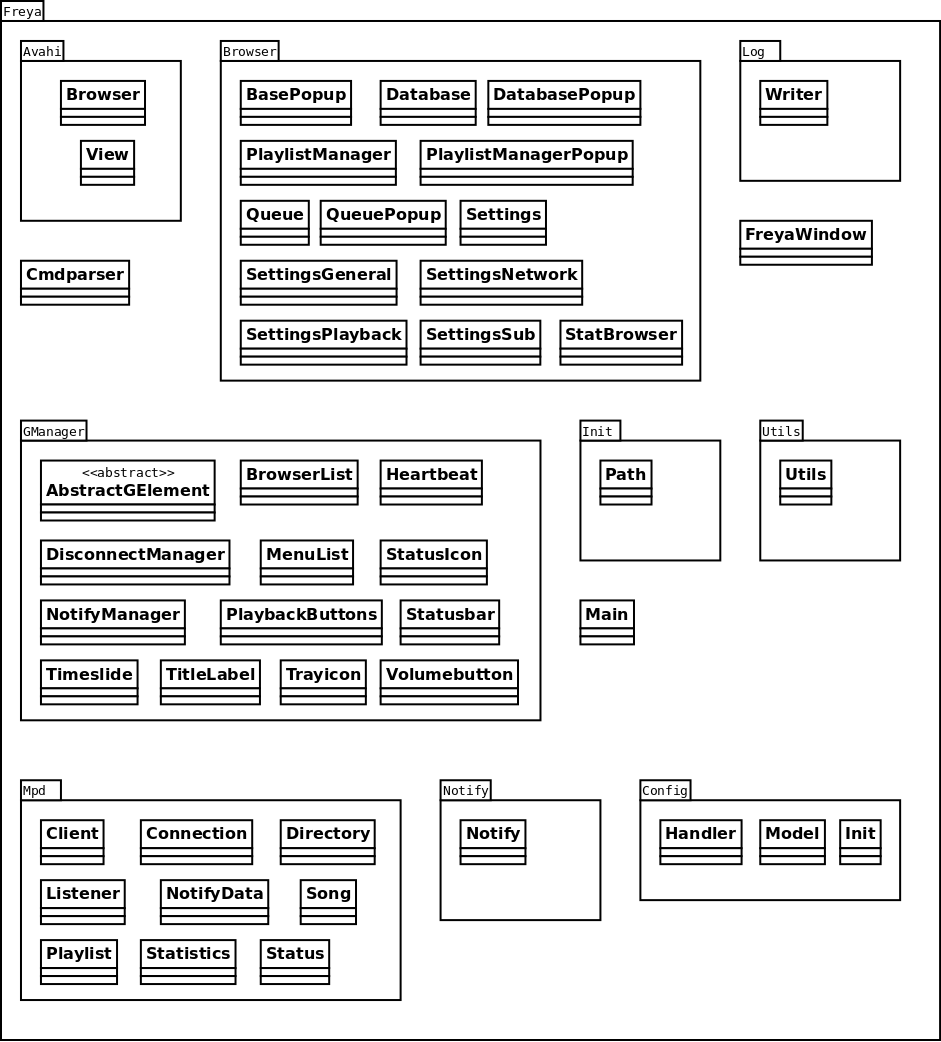
\includegraphics[scale=0.21]{Namespace_Uebersicht.png}
    \caption{Die MPD Namespaces im Überblick}
    \label{dd_namespaces}
\end{figure}

\section{,,Das Problem''}

Da die grundlegende Funktionsweise des MPD Server auf einer Client Server Architektur beruht, muss der MPD Client
verschiedene Kommandos wie zum Beispiel play, pause, listplaylists etc. an den Server schicken
und zur gleichen Zeit aber auch auf Änderungen reagieren können, d.h. zum Beispiel wenn sich die Lautstärke ändert,
da jederzeit auch andere Clients oder Server den MPD internen Zustand ändern können.
Diese Änderungen müssen auch anderen Programmteilen bekannt gemacht werden. (Observer Pattern)
\\
Der Client sollte im ,,idle''-Mode möglichst keine Ressourcen verschwenden und auch beim 
disconnecten und conntecten die entprechenden Änderungen anderen Teilen des Programms mitteilen
können(Observer Pattern)\footnote{http://de.wikipedia.org/wiki/Observer\_(Entwurfsmuster)}. 
\\

Das MPD Protokoll \footnote{http://www.musicpd.org/doc/protocol/index.html} bietet folgende Möglichkeiten das zu realisieren
\begin{description}
    \item [Periodisch] (zB. alle 500ms) das ,,status'' command absetzen und nach Bedarf auch commands wie ,,currentsong''
        senden
        \\
        \emph{Problem:} Bei langsamen Netzwerkverbindungen erzeugt dies unnötige Netzwerklast 
        Prinzipiell würde sich auf diese Art jedoch die z. B. Musik Bitrate anzeigen lassen, es ist jedoch ein
        wenig komfortabler Weg da hier wieder einmal das Rad neu erfunden werden müsste.
    \item [Nutzung der ,,idle'' und ,,noidle'' commands:]
        ,,idle'' versetzt die Verbindung zum Server in einen Schlafzustand, sobald ,,events'' wie 'player' (also z. B. pause oder play) 
        eintreten, wacht die Verbindung aus diesem Zustand auf und sendet an den Client eine Liste der Events die aufgetreten sind:

\begin{figure}[h!]
    \lstinputlisting[language=bash]{state.txt}
\caption{Eine Beispielantwort des MPD Servers}
\label{dd_state}
\end{figure}
>>>>>>> katze:doc/architecture/Doku/DesignDokument.tex

        Einschränkung: Während die Verbindung im idle mode ist kann kein reguläres Kommando wie ,,play'' gesendet werden!
        Sollte man es doch tun wird man vom Server augenblicklich mit einem Disconnect belohnt.
        Die einzige Möglichkeit aus dem idle mode aufzuwachen ist das 'noidle' command das gesendet werden
        kann während die verbindung schlafen gelegt wurde.
        Jedoch gibt es auch hier ein Problem, denn das ,,idle'' command blockiert, sprich es sendet kein ,,OK'' zurück zum Sender.
        Ein Warten auf dieses ,,OK'' würde mit den Wunsch eine bedienbare Oberfläche zu haben kollidieren.
\end{description}

Prinzipiell gibt es 2 Möglichkeiten dieses Problem zu lösen:
\begin{itemize}
    \item Man hält zwei Verbindungen zum Server, eine die Kommandos sendet, eine die stets im ,,idle'' mode liegt,
        Für die Realisierung müssten Threads herangezogen werden. Ein Thread würde dann im Hintergrund auf events lauschen,
        der andere würde zum Abschicken der Kommandos benutzt werden.
        Problem: Es müssen 2 Verbindungen gehandelt werden, was wiederum ein Mehraufwand an Code bedeutet.
        Desweiteren werden Threads benötigt die auch in anderen Bereichen des Programms Lockingmechanismen bedeuten würden.
    \item Man hält eine asynchrone verbindung zu dem server.
        Diese kann das 'idle' command zum server schicken, returned aber sofort. Um nun eine Liste der events zu bekommen setzt man 
        einen ,,Watchdog''auf die asynchrone verbindung an (Vergleiche dazu den Systemaufrug 'man 3 poll'). Da poll() ebenfalls den
        aufrufenden Prozess blockiert, wird Glib::signal\_io() benutzt, das sich in den laufenden MainLoop (*) einhängt und eine 
        Callbackfunktion aufruft sobald auf der verbindung etwas interessantes passiert. Da während des Wartens der MainLoop weiterarbeitet,
        bleibt die GUI (und andere Module) aktiv und benutzbar.
        Problem: Vor dem Senden eines Kommandos wie ,,play'' muss der idle mode verlassen werden.
        Lösung: Man kann das ,,noidle'' Kommando zum verlassen senden, und nach dem Absenden des eigentlichen Kommandos wieder den idle-mode betreten.
\end{itemize}

%* MainLoop: Vergleiche Event Dispatcher auf wikipedia. Gtk+ benutzt intern einen MainLoop um auf die user ergebnisse reagieren zu können.
%            Desweiteren kann man eigene events in den Loop einhängen, wie beispielsweise ein Timeoutevent das alle 500ms ausgeführ

\lstinputlisting[language=bash]{telnet.txt}


Die Idee zu dieser Implementierung (speziell das Benutzen einer asynchronen Verbindung), kommt von ,,ncmpc'',
der inoffiziellen offiziellen Referenzimplementierung des MPD Mit-Authors \emph{Max Kellermann}.
Vergleiche \href{http://mpd.wikia.com/wiki/Client:Ncmpc}{ncmpc quellcode}: src/gidle.c und src/mpdclient.c


\section{Aufbau des Clients}

Aus den oben genannten Anforderungen kann eine grobe Architektur abgeleitet werden.
Zur Realisierung des Observerpatterns wird die sigc++ library benutzt die mit Gtkmm kommt.
Es wird empfohlen die Einführung bis einschließlich Kapitel 2 zu lesen:
\begin{itemize}
\item \url{http://developer.gnome.org/libsigc++-tutorial/stable/ch01.html}
\end{itemize}
Die ersten Einsätze werden auch noch tiefer erklärt.


\subsection{Hauptklassen}
\begin{figure}[htb!]
	\centering
        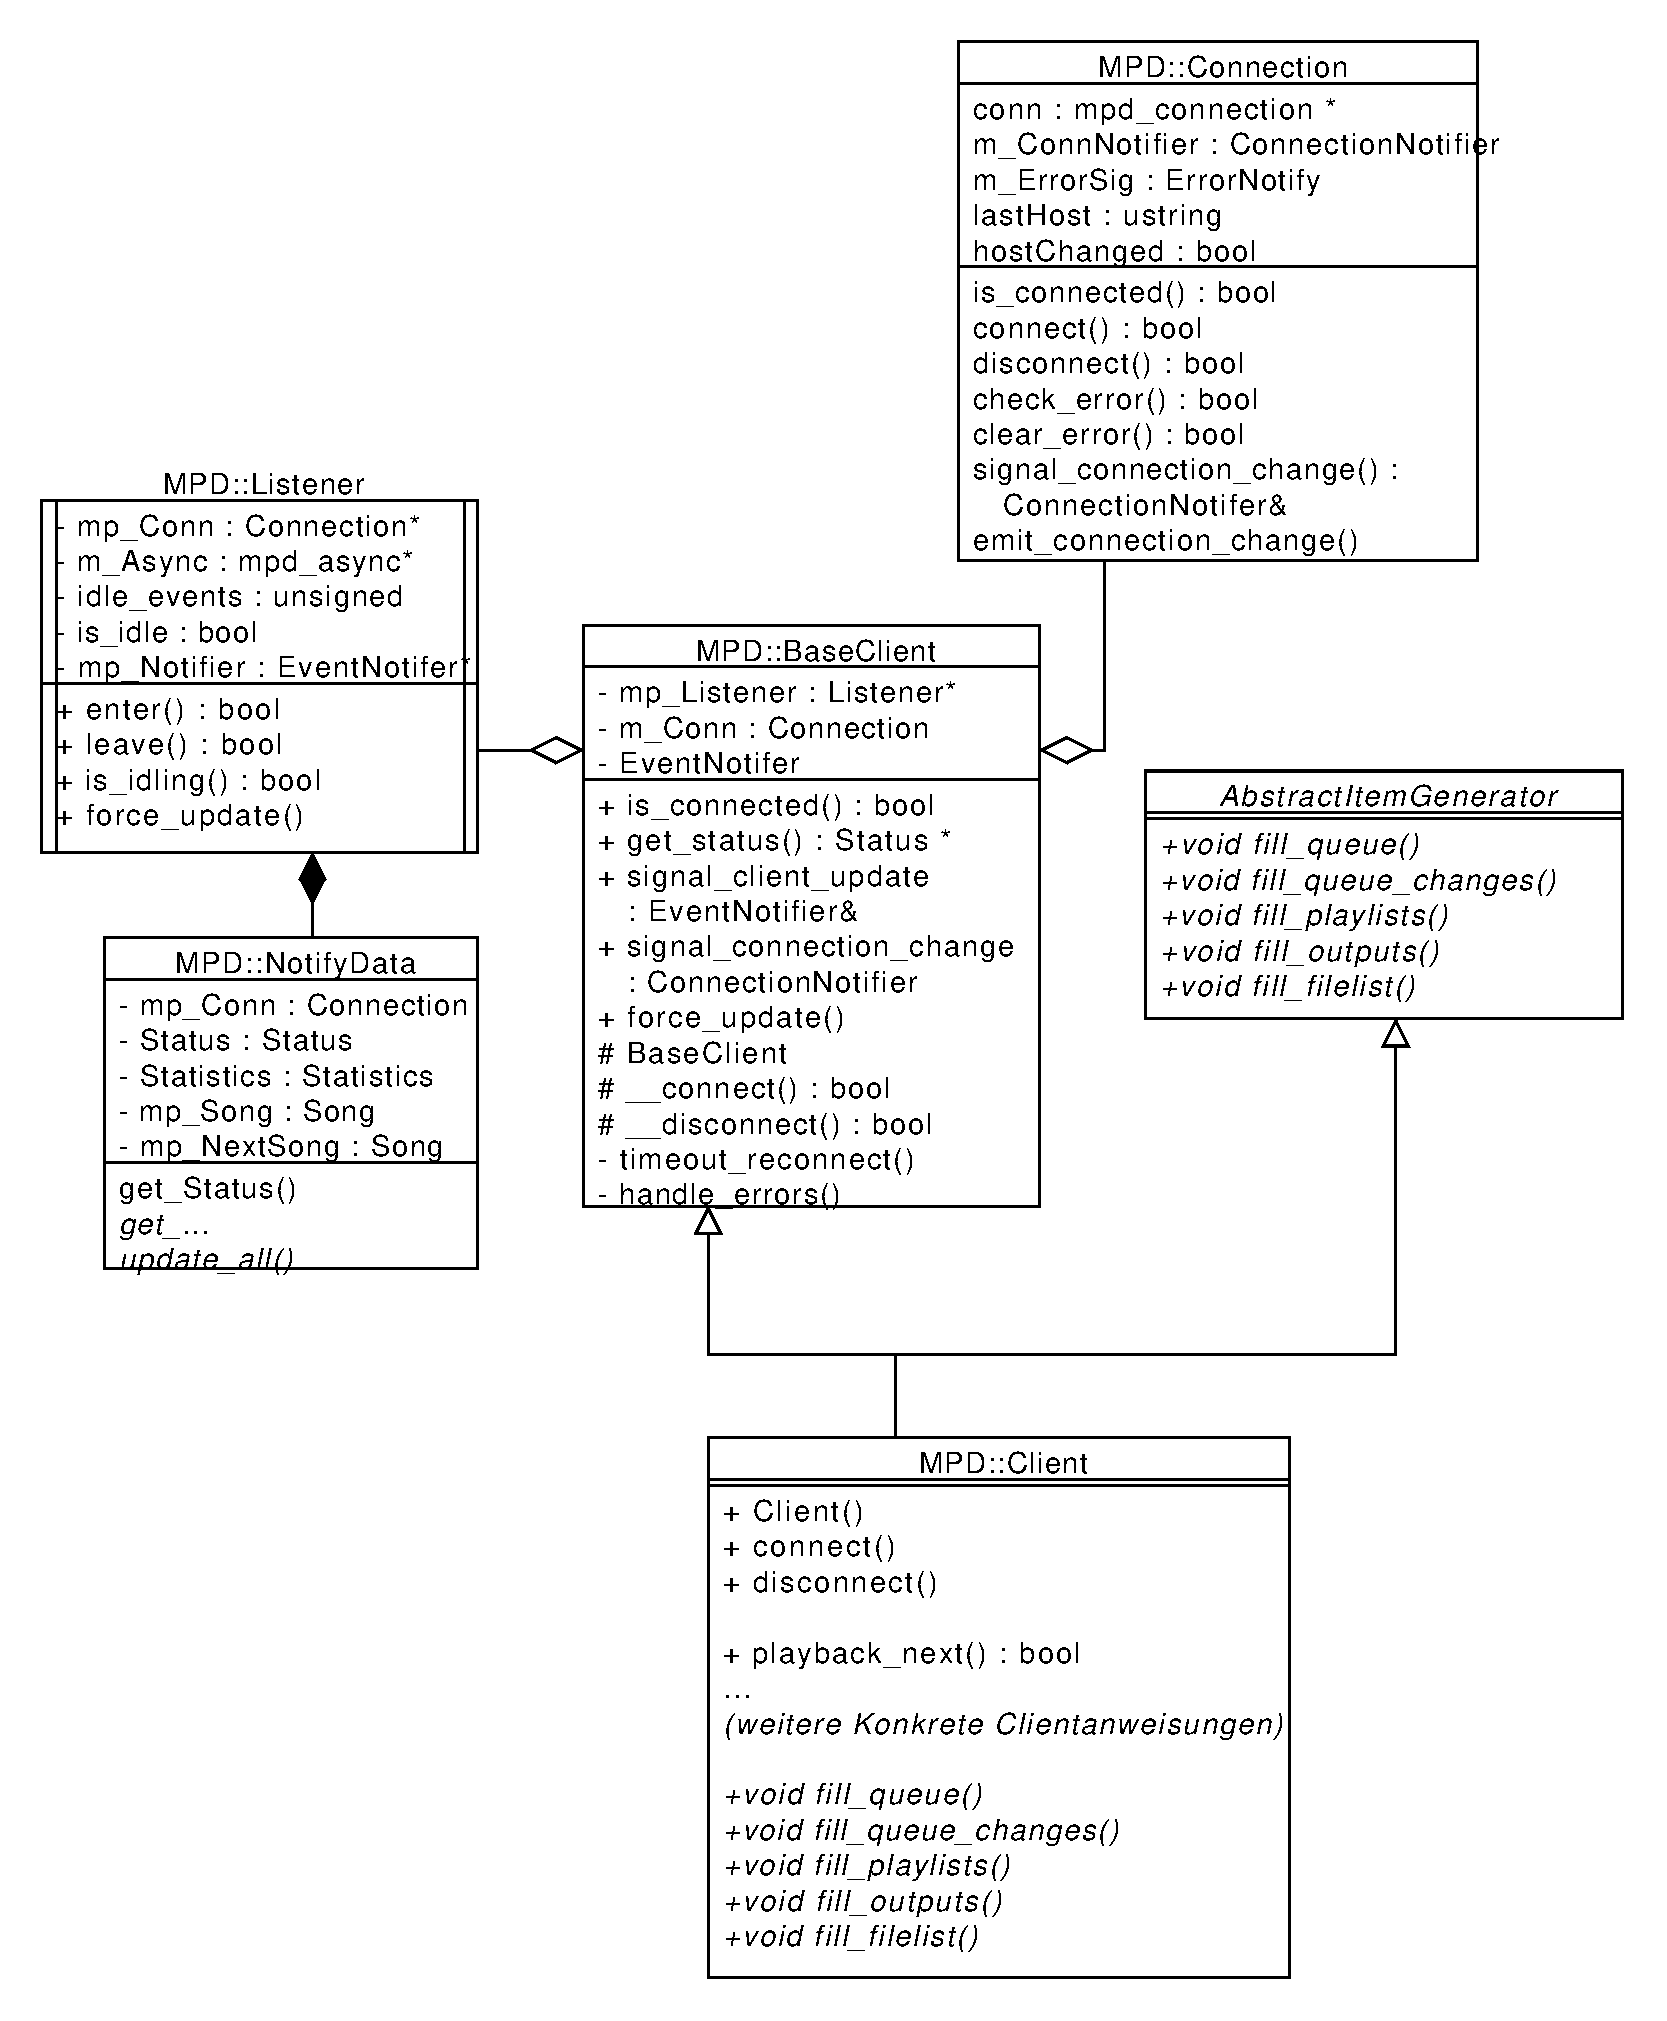
\includegraphics[scale=0.5]{ClientCollab.pdf}
	\caption{Übersichtsklassendiagramm zur Clientstruktur}
	\label{class_client_all}
\end{figure}

\subsubsection{Listener}
Der Listener verwaltet alles was mit dem Betreten und Verlassen des ,,Idlemodes'' und den damit verbundenen Events
zu tun hat. Er setzt den eingangs beschriebenen ,,Watchdog'' auf die asynchrone Verbindung an,
und ,,parst'' die entsprechenden Antworten des Servers von Hand. 
\\
\\
Es folgt eine Liste aller möglichen Events die von libmpdclient definiert werden.
Die Aktionen die passieren müssen, damit diese eintreten, stehen in Klammern.
\begin{itemize}
    \item \small MPD\_IDLE\_DATABASE \it(Datenbank hat sich geändert)\rm
    \item \small MPD\_IDLE\_STORED\_PLAYLIST \it(Änderung an den Playlisten)\rm
    \item \small MPD\_IDLE\_QUEUE \it(Änderung an der Queue: Clear, Add, Remove)\rm
    \item \small MPD\_IDLE\_PLAYER \it(Pause,Stop,Play,Next,Stop,Previous,Seek)\rm
    \item \small MPD\_IDLE\_MIXER \it(Änderung an der Lautstärke)\rm
    \item \small MPD\_IDLE\_OUTPUT \it(An/Ausschalten eines Outputs)\rm
    \item \small MPD\_IDLE\_OPTIONS \it(Random,Repeat,Single,Consume)\rm
    \item \small MPD\_IDLE\_UPDATE \it(Datenbankupdate/rescan wurde gestartet)\rm
\end{itemize}
\normalsize
Bei der Instanzierung des Listeners soll das \textit{sigc::signal} welches das Clientupdate darstellt übergeben werden.
Zudem benötigt der Listener eine Referenz auf MPD::Connection um an die darunter liegende asynchrone Verbindung zu kommen.  
\begin{verbatim}
  Listener(EventNotifier& Notifier, Connection& sync_conn);
\end{verbatim}

Eine weitere Aufgabe des Listeners ist es, das Model MPD::NotifyData aktuell zu halten. Siehe dazu auch MPD::NotifyData.
Bemerkt der Listener Events so ruft er emit() auf dem übergebenen \textit{sigc::signal} auf,
und übergibt als Parameter das aufgetretene Event, sowie eine Instanz von MPD::NotifyData.
\footnote{Als spätere Optimierung könnte das aufgetretene Event übergeben werden um selektiv Daten ,,upzudaten''; Sprich bei einer Lautstärkeänderung muss kein neues Statistikobjekt geholt werden.}
\\
Es folgt eine Liste von Funktionen die der Listener mindestens haben soll.
\\
enter() tritt in den ,,Idlemode'' ein. Es ist ab diesem Punkt nicht mehr erlaubt Kommandos zu senden.
leave() ist das genaue Gegenteil von enter() und verlässt den ,,Idlemode'' sodass Kommandos gesendet werden können.  
is\_idling() sollte selbsterklärend sein.
\begin{verbatim}
       bool enter(void);
       void leave(void);
       bool is_idling(void);
\end{verbatim}

Es soll zudem eine force\_update() Funktion geben die ,,künstlich'' alle Events auslöst.
Dies ist nützlich bei der Initialisierung, bzw. bei ,,Reconnectvorgängen'', wenn die GUI gezwungen werden
soll sich zu updaten.
\begin{verbatim}
       void force_update(void);
\end{verbatim}

\subsubsection{Connection}
\begin{figure}[htb!]
	\centering
        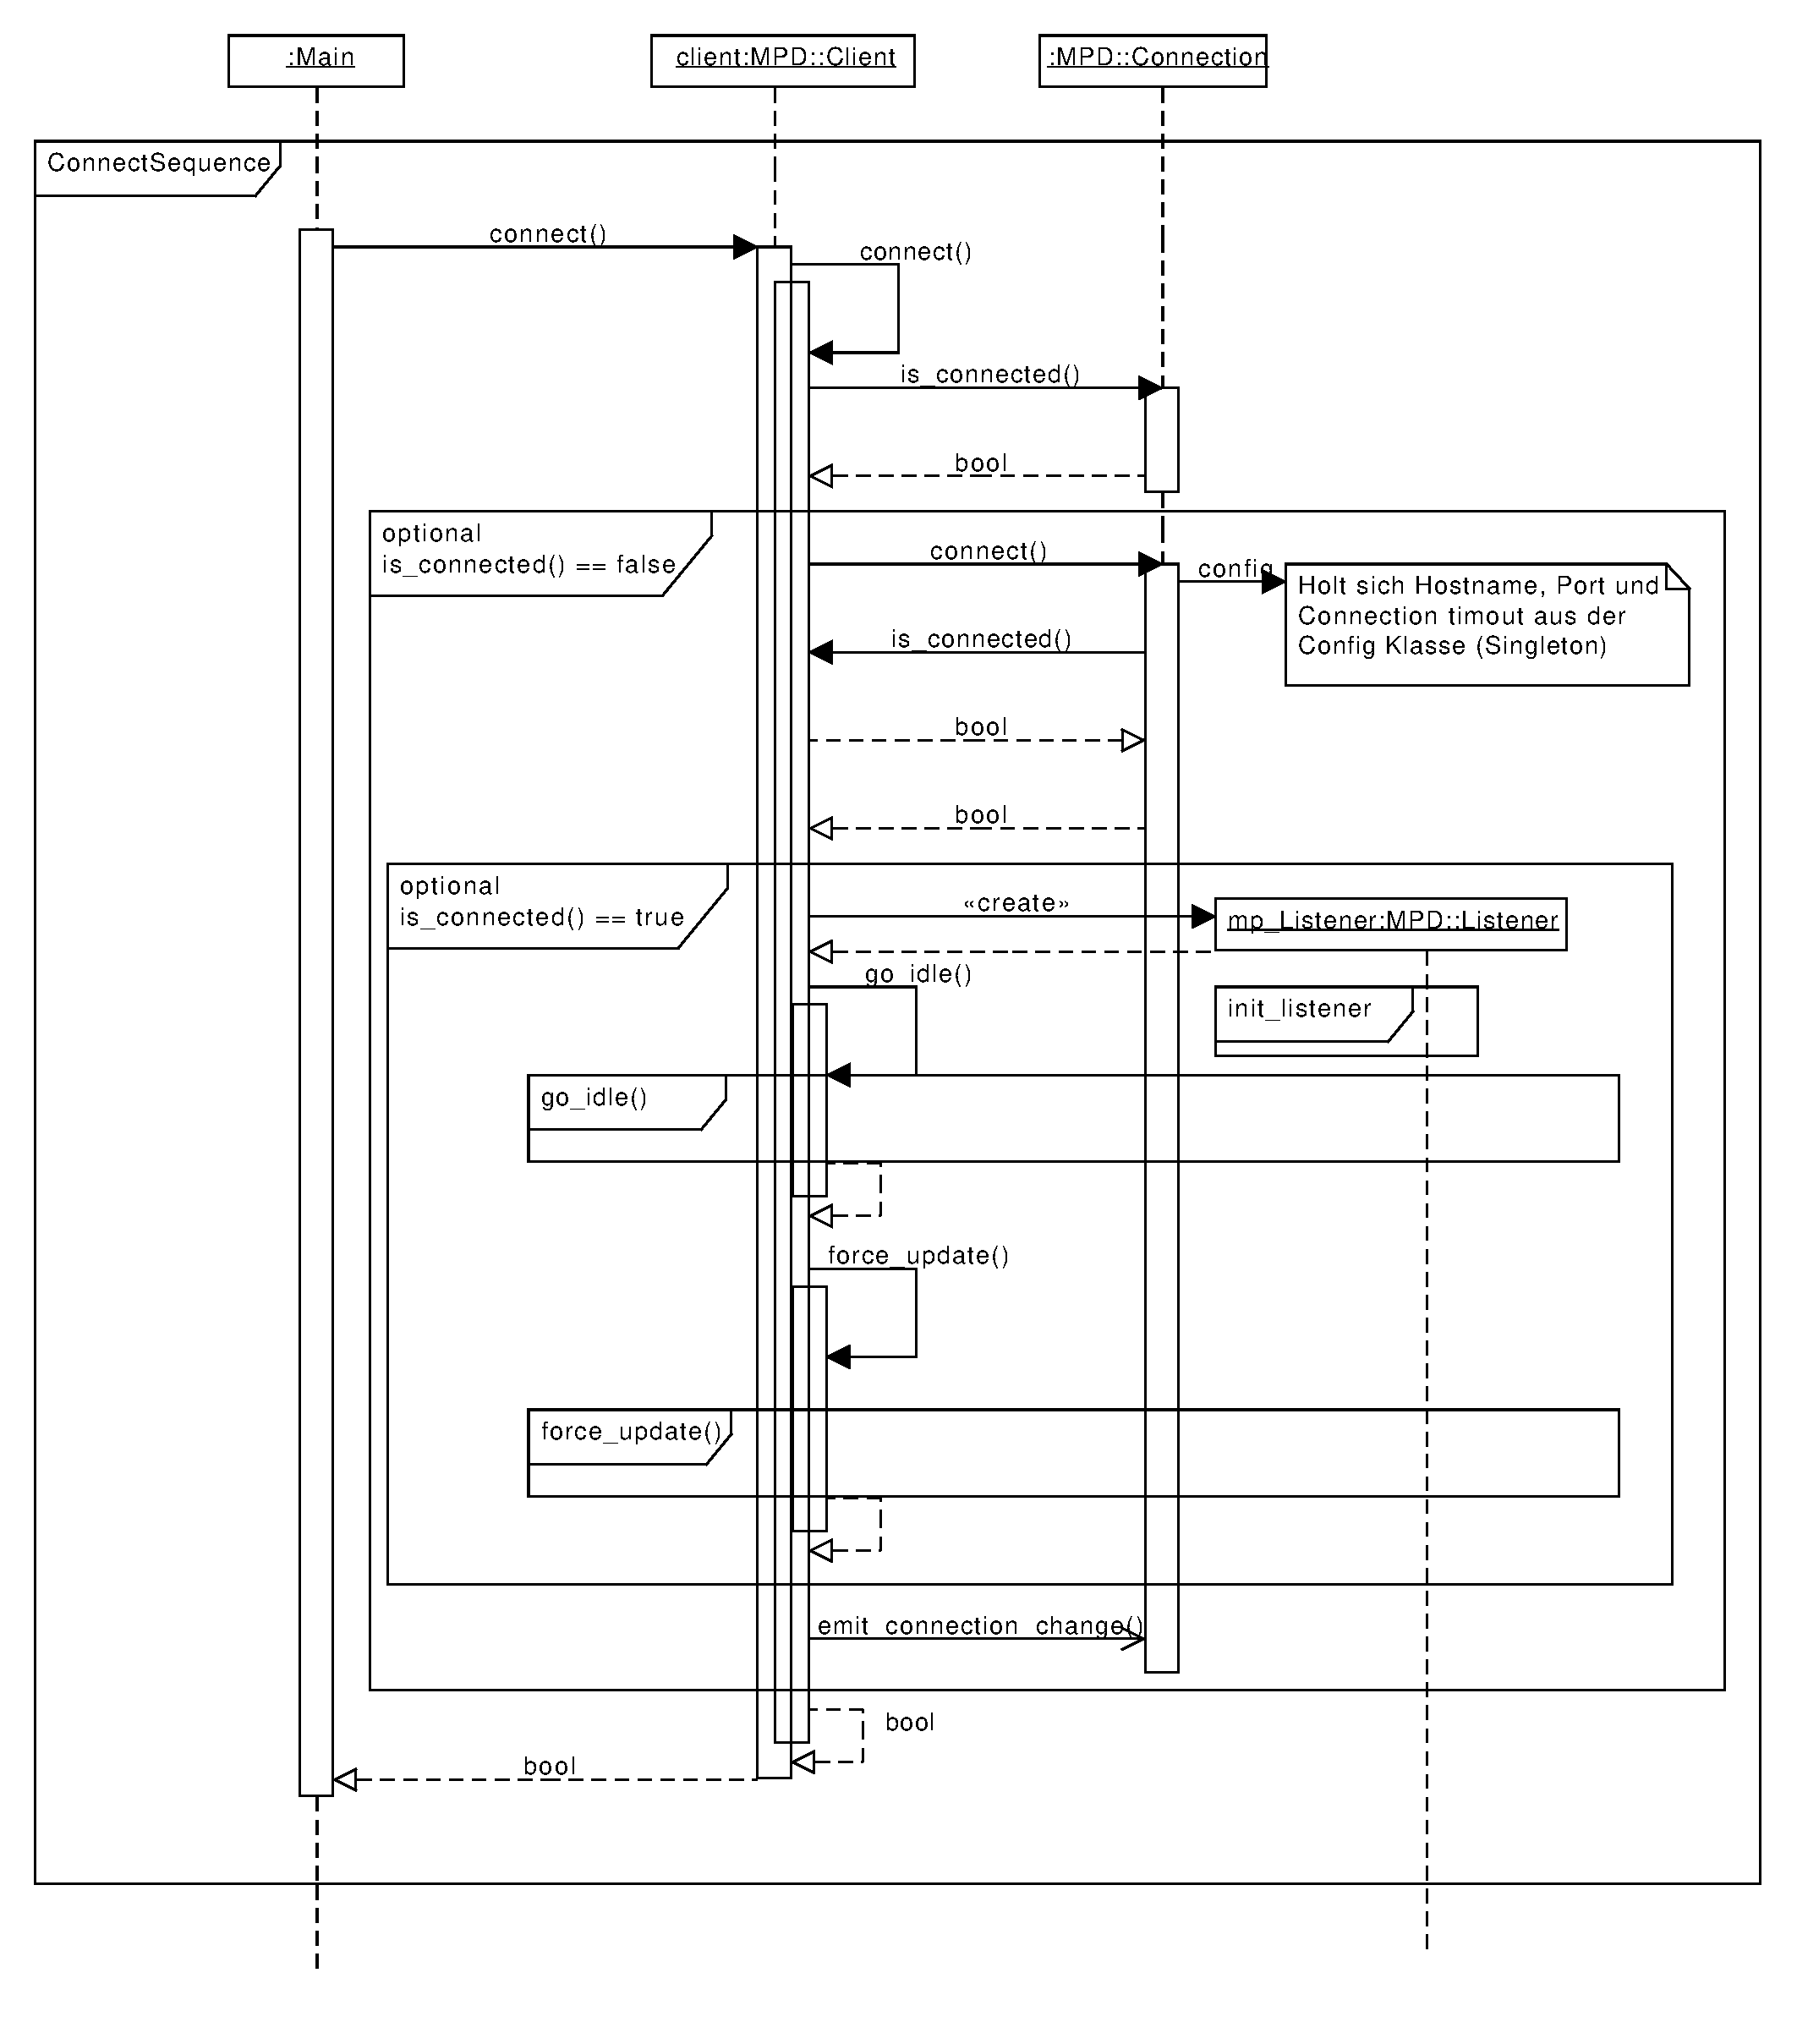
\includegraphics[scale=0.5]{ConnectSequence.pdf}
	\caption{Sequenzdiagramm zum Verbindungsaufbau}
	\label{seq_client_connect}
\end{figure}
Diese Klasse stellt eine Art Wrapper um die \textit{mpd\_connection}
\footnote{http://www.musicpd.org/doc/libmpdclient/connection\_8h.html} Struktur von libmpdclient da.
Sie bietet die ,,eigentlichen'' connect() und disconnect() Methoden die letzlich \textit{mpd\_connection\_new()} bzw. \textit{mpd\_connectio\_free()} aufrufen. Siehe \ref{seq_client_connect} für den detaillierten Verbindungsablauf. Die benötigten Verbindungsdaten (Host, Port, Timeout in Sekunden) holt sich MPD::Connection aus der Config.
\\
Sie hält zudem den letzten Host als Membervariable um feststellen zu können ob sich dieser zwischen 
zwei Verbindungsvorgängen geändert hat. Desweiteren bietet sie eine Schnittstelle um andere Klassen über Fehler in der Verbindung informieren zu lassen (signal\_error()), bzw. um sie zu ,,reparieren'' (clear\_error()).
\\
Es folgt eine Liste von Funktionen die mindestens vorhanden sein sollten.
Ein boolean-Rückgabewert von true zeigt stets Erfolg an.
\\
connect() soll die eigentliche Verbindung herstellen, disconnect() löscht die Verbindung wieder.
get\_connection() liefert einen Pointer auf die darunter liegende C-Struktur.
Alle 3 Funktionen prüfen zudem intern bereits auf Fehler. 
\begin{verbatim}
    bool is_connected(void);
    bool connect(void);
    bool disconnect(void);
\end{verbatim}

Zur Implementierung konkreter Kommandos wird die darunterliegende C-Struktur benötigt.
\textbf{Siehe auch:} AbstractClientExtension
\begin{verbatim}
    mpd_connection * get_connection(void);
\end{verbatim}

Die Connectionklasse soll zudem Schnittstellen bieten um sich für Fehler- und Verbindungsänderungen
zu registrieren. 
Auf den Rückgabewert der folgenden Funktionen kann sigc::signal::connect() aufgerufen werden,
um einen Funktionspointer zu registrieren der aufgerufen wird sobald ein Fehler eintritt,
bzw. sich die Verbindung ändert. Die Schnittstellen sollen wie folgt aussehen:
\begin{verbatim}
  typedef sigc::signal<void, bool,mpd_error> ErrorNotify;
  typedef sigc::signal<void,bool,bool> ConnectionNotifier;
    
  ErrorNotify& signal_error(void);
  ConnectionNotifier& signal_connection_change(void)
\end{verbatim}

Die Prototypen entsprechen stets den Templateargumenten in den typedefs:
\begin{verbatim}
  void error_handler(bool is_fatal, mpd_error err_code);
  void conn_change_handler(bool server_changed, bool is_connected); 
\end{verbatim} 

Siehe MPD::BaseClient weiter unten für ein Beispiel wie eine Callbackfunktion registriert wird.
\\
libmpdclient verbietet es weitere Kommandos an den Server zu senden wenn vorher ein Fehler passiert ist.
Fehler müssen zuerst mit \emph{mpd\_connection\_clear\_error()} ,,bereinigt'' werden, 
dies tut check\_error(). Die Funktion wird normal nicht selbst aufgerufen, da sie von allen anderen Funktionen der Klasse
implizit aufgerufen wird. Ist ein Fehler passiert so werden alle Klienten die sich zuvor
mit signal\_error() registriert haben benachrichtigt. 
\begin{verbatim}
  bool check_error(void);
\end{verbatim}

\begin{figure}[htb!]
	\centering
        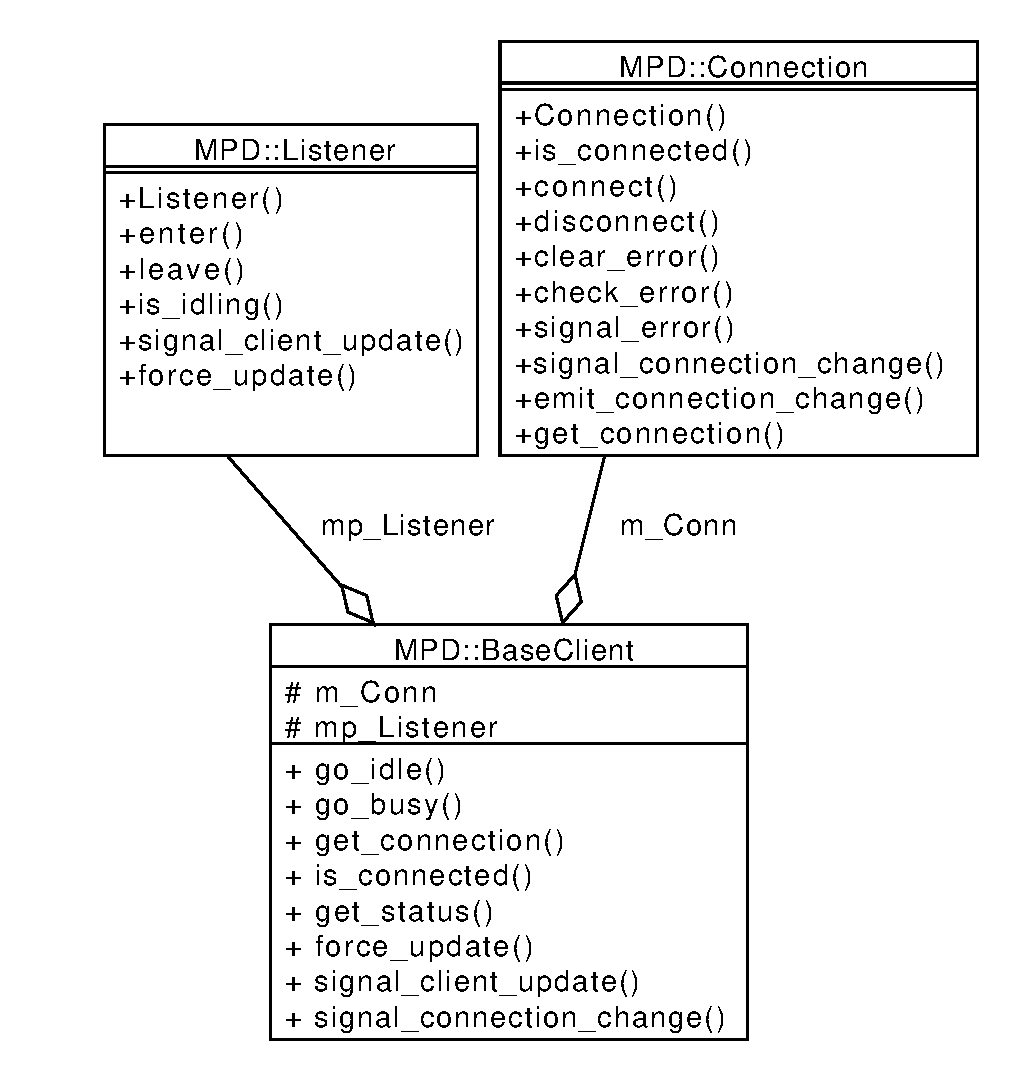
\includegraphics[scale=0.55]{BaseClientCollab.pdf}
	\caption{Klassendiagramm zu BaseClient}
	\label{collab_base_client}
\end{figure}

\subsubsection{BaseClient}
Diese Klasse bildet die Basis zum eigentlichen Client. Sie kann nicht direkt instanziert werden, da
der Konstruktor protected sein soll.
Sie verwaltet administrative Tätigkeiten wie den eigentlichen Verbindungsaufbau \ref{seq_client_connect} an sich. 
Desweiteren bietet die Klasse einfache Methoden zum Eintreten (go\_idle()) und Verlassen (go\_busy()) des ,,Idlemodes'' an.
Geht die Verbindung verloren, ohne dass \emph{\_\_disconnect()} explizit aufgerufen wurde, so wird versucht sich periodisch zu reconnecten.
Das Intervall in dem diese Versuche geschehen sollen, soll von ,,settings.connection.reconnectinterval'' gelesen werden.
\\
\\
\textbf{Siehe auch:} AbstractClientExtension
\\
MPD::BaseClient soll mindestens folgende public Methoden bieten:
\\
Gibt eine Referenz auf das zugrunde liegende MPD::Connection Objekt zurück. 
Siehe AbstractClientExtension für eine detailliertere Erklärung.
\\
\begin{verbatim}
  Connection& get_connection(void);
\end{verbatim}

Gibt \textit{true} zurück wenn eine Verbindung besteht.
\begin{verbatim}
   bool is_connected(void);
\end{verbatim}

Die get\_status() Funktion soll den letzten aktuellen MPD::Status zurückliefern,
oder \emph{NULL} falls nicht verbunden. Es soll garantiert sein, dass stets ein MPD::Status vorliegt,
wenn is\_connected() wahr ergibt.
\begin{verbatim}        
   Status * get_status(void);
\end{verbatim}

Die folgenden Methoden bieten eine Möglichkeit sich für Clientevents (signal\_client\_update()),
 bzw. für Verbindungsänderungen (signal\_connection\_change()) zu registrieren. 
\begin{verbatim}
  typedef sigc::signal<void,mpd_idle,MPD::NotifyData&> EventNotifier;
  EventNotifier& signal_client_update(void);
        
  typedef sigc::signal<void,bool,bool> ConnectionNotifier;
  ConnectionNotifier& signal_connection_change(void);
\end{verbatim}

Registrieren kann man sich über die sigc::signal::connect() Methode:
\begin{verbatim}
 // Callback Funktion wird bei jedem eingetretenen Event aufgerufen
 void on_client_update(enum mpd_idle event, MPD::NotifyData& data)
 {
    // Tue etwas bei einem 'player' event
    if(event == MPD_IDLE_PLAYER)
    {
        // Gib den Namen des aktuellen Songs aus
        cerr << data.get_song().get_path() << endl;
    }
 }

 // Registrieren der Callbackfunktion
 // - Ableiten von AbstractClientUser macht dies automatisch
 m_Client.signal_client_update().connect(sigc::ptr_fun(on_client_update));
\end{verbatim}

Folgende 3 Funktionen funktionieren genau wie enter(), leave() und force\_update() des Listeners,
allerdings prüfen sie mit Connection::check\_error() vorher stets auf Fehler.
\begin{verbatim}
  void go_idle(void);
  void go_busy(void);
  void force_update(void);
\end{verbatim}

%
%
%
% Zustands oder Sequenzdiagram zum Ausfürehn eines beliebigen Kommandos
% Sprich: go_busy( ) -> send command -> go_idle( )
%
\subsubsection{Client}
Der Client erbt von BaseClient und implementiert konkrete Kommandos wie ,,play'',,,random'' etc.
Er bietet zudem Schnittstellen zur Befüllung der Datenbank, der Queue und des Playlistmanagers indem 
er die abstrakte Klasse \emph{AbstractClientExtension} ausimplementiert.
Er bietet die Methoden connect() und disconnect() die letzendlich von Anwendern der Clientklasse zum Verbinden und Trennen genutzt werden. 
Ist in der config ,,settings.connection.autoconnect'' gesetzt, so connected er sich automatisch.
\\
\\
connect() und disconnect() stellen die öffentliche Schnittstelle zum Verbinden dar.
Sie rufen intern lediglich \_\_connect() bzw. \_\_disconnect() von MPD::BaseClient auf.
\begin{verbatim}
    void connect(void);
    void disconnect(void);
\end{verbatim}

Der Client soll eine Reihe von Kommandos bereitstellen um das Playback zu kontrollieren.
Die ersten 5 der folgenden Funktionen sollten relativ klar sein. 
Zu playback\_pause() sei angemerkt, dass es bei Wiedergabe anhält und bei keiner Wiedergabe wie playback\_play() funktioniert.
playback\_seek() springt in den Song mit der ID song\_id an die Stelle abs\_time in Sekunden.
Die ID des momentan spielenden Songs kann durch get\_status() gefunden werden.
Alle Funktionen, mit Ausnahme von playback\_crossfade), lösen ein ,,player'' Event aus. 
playback\_crossfade löst hingegen ein ,,options'' Event aus.
\begin{verbatim}
    void playback_next(void);
    void playback_prev(void);
    void playback_stop(void);
    void playback_play(void);
    void playback_crossfade(unsigned seconds);    
    void playback_pause(void);
    void playback_seek(unsigned song_id, unsigned abs_time);
    void playback_song_at_id(unsigned song_id);
\end{verbatim}

Die folgenden Funktionen dienen dazu jeweils die \it random, consume, repeat\rm und \textit{single}-modi umzuschalten.
Alle lösen ein ,,options'' Event aus.
\begin{verbatim}
    void toggle_random(void);
    void toggle_consume(void);
    void toggle_repeat(void);
    void toggle_single(void);
\end{verbatim}

Desweiteren sollten Methoden zum Bearbeiten der Queue vorhanden sein.
\begin{itemize}
    \item \textbf{queue\_add():} Fügt rekursiv den Pfad in der Datenbank hinzu. queue\_add(``/'') entspricht der ganzen Datenbank.
    \item \textbf{queue\_clear():} Leert die gesamte Queue.
    \item \textbf{queue\_delete():} Leert den Song ander Position 'pos'
    \item \textbf{queue\_save\_as\_playlist():} Speichert die aktuelle Queue als Playlist mit dem Namen 'name'
\end{itemize}
\begin{verbatim}
    void queue_add(const char * url);
    void queue_clear(void);
    void queue_delete(unsigned pos);
    void queue_save_as_playlist(const char * name);
\end{verbatim}

database\_update() sendet MPD Server Hinweis um DB zu aktualisieren.
database\_rescan() sendet MPD Server Hinweis um DB neu einzulesen (teuer).
\begin{verbatim}
    void database_update(const char * path);
    void database_rescan(const char * path);
\end{verbatim}

Setzen des ,,volumes'' von 0 bis 100\%.
Die Abfrage des Volumes kann über get\_status() erfolgen.
\begin{verbatim}
    void set_volume(unsigned vol);
\end{verbatim}

Folgende Funktionen sollen von \emph{AbstractItemGenerator} voll implementiert werden.
Siehe daher \emph{AbstractItemGenerator} für eine genaue Erklärung.
\begin{verbatim}
    void fill_queue(AbstractItemlist& data_model);
    void fill_queue_changes(AbstractItemlist& data_model,
                            unsigned last_version,
                            unsigned& first_pos);
    void fill_playlists(AbstractItemlist& data_model);
    void fill_outputs(AbstractItemlist& data_model);
    void fill_filelist(AbstractItemlist& data_model, const char * path);
\end{verbatim}

\subsubsection{NotifyData}
Speichert den aktuellen Status, den aktuellen Song und die aktuelle Datenbankstatistik.
Bietet zudem eine Funktion um entsprechende Daten bei Aufruf zu ,,updaten''.
Die Klasse gehört nach dem MVC Pattern somit der Modelebene an.
Der Listener instanziert NotifyData im Konstruktor und gibt an wann sich dieser ,,updaten'' soll (über update\_all()).
\\        

Die folgenden 2 Funktionen garantieren einen validen Rückgabewert, solange eine Verbindung besteht:
\begin{verbatim}
    Status& get_status(void);
    Statistics& get_statistics(void);
\end{verbatim}

\textbf{Anmerkung:} Die folgenden 2 Funktionen sollen NULL zurückgeben können, falls beispielsweise
nichts wiedergegeben wird, oder man im ,,\textit{Singlemode}'' ist.
get\_song() liefert den aktuell spielenden MPD::Song, oder \emph{NULL}.
get\_next\_song() liefert den als nächstes spielenden MPD::Song oder \emph{NULL}.
\begin{verbatim} 
    Song * get_song(void);
    Song * get_next_song(void);
\end{verbatim}

Die update\_all() sollte nur vom Listener aufgerufen werden. Sie aktualisiert den internen Zustand
von NotifyData.
\begin{verbatim}
    void update_all(unsigned event);
\end{verbatim}


\subsection{Weitere Klassen}
Desweiteren gibt es einige weitere Klassen die am Rande eine Rolle spielen,
und meist objektorientierte Wrapperklassen für die C-Strukturen von libmpdclient bereitstellen,
oder im Falle von MPD::AudioOutput und MPD::Playlist eigene Clientkommandos implementieren.

\subsubsection{Song}

Die Song Klasse ist ein Wrapper für mpd\_song Struktur und die dazugehörigen Funktion von libmpdclient. 
MPD::Song soll alle Funktionen von libmpdclient \footnote{http://www.musicpd.org/doc/libmpdclient/song\_8h.html} anbieten.
Diese werden hier nur aufgelistet aber nicht erklärt da sie genau wie ihre Vorbilder funktionieren sollen:

\begin{verbatim}
    const char * get_path(void);
    const char * get_tag(enum mpd_tag_type type, unsigned idx);
    unsigned get_duration(void);
    time_t get_last_modified(void);
    void set_pos(unsigned pos);
    unsigned get_pos(void);
    unsigned get_id(void);
\end{verbatim}

MPD::Song soll zudem eine Funktion bieten um die Metadaten des Songs in einer ,,sprintf'' änhlichen Art als String zurückzuliefern:
\begin{verbatim}
    Glib::ustring song_format(const char* format, bool markup=true);
\end{verbatim}

Ein beispielhafter Aufruf:
\begin{verbatim}
    SomeSong.song_format("Artist is by ${artist}") 
\end{verbatim}

Die Escapestrings die dabei unterstützt werden sollen entsprechen in etwa der \textit{mpd\_tag\_type} Enumeration vom libmpdclient.\footnote{http://www.musicpd.org/doc/libmpdclient/tag\_8h.html\#a3e0e0c332f17c6570ffdf788a685adbf}
Die unterstützten Typen sind somit: \it artist, title, album, track, name, data, album\_artist, genre, composer, performer, comment, disc\rm.
Ist ein Escapestring nicht bekannt, so wird er nicht escaped. Ist der ,,tag'' nicht vorhanden, soll mit ,,unknown'' escaped werden.
\\
Diese Klasse gehört nach dem MVC Paradigma zur Modelschicht.

\subsubsection{Directory}
Die Directory Klasse ist ein Wrapper für mpd\_directory C-Strukutr. Diese wird als Anzeige für ein Verzeichniss benutzt, jedoch nicht als Container für andere Elemente.

Da MPD::Directory die abstrakte Klasse AbstractComposite erweitert muss als
einzige öffentliche Funktion get\_path() implementiert werden:
\begin{verbatim}
    void get_path(void);
\end{verbatim}

Diese Klasse gehört nach dem MVC Paradigma zur Modelschicht.

\newpage
\subsubsection{Statistics}
Die Statistics Klasse ist ein Wrapper für mpd\_stats und
implementiert somit gemäß \url{http://www.musicpd.org/doc/libmpdclient/stats\_8h.html}
folgende Funktionen:
\begin{verbatim}
    unsigned get_number_of_artists(void);
    unsigned get_number_of_albums(void);
    unsigned get_number_of_songs(void);
    unsigned long get_uptime(void);
    unsigned long get_db_update_time(void);
    unsigned long get_play_time(void);
    unsigned long get_db_play_time(void);
\end{verbatim}

Diese Klasse gehört nach dem MVC Paradigma zur Modelschicht.

\subsubsection{Playlist}
Die Playlist Klasse ist Wrapper für die mpd\_playlist Struktur und
implementiert von \url{http://www.musicpd.org/doc/libmpdclient/playlist\_8h.html} folgende Funktionen:
\begin{verbatim}
    const char * get_path(void);
    time_t get_last_modified(void);
\end{verbatim}

Die Klasse bietet desweiteren  Funktionen zum:
\begin{itemize}
\item Entfernen der Playlist vom Server (Das Playlistobjekt ist danach invalid):
\begin{verbatim}
    void remove(void);
\end{verbatim}

\item Laden der Playlist in die Queue:
\begin{verbatim}
    void load(void);
\end{verbatim}

\item Umbennen der Playlist:
\begin{verbatim}
    void rename(const char * new\_name);
\end{verbatim}

\item Hinzufügen von Songs zur Playlist:
\begin{verbatim}
    void add_song(const char * uri);
    void add_song(MPD::Song& song);
\end{verbatim}
\end{itemize}
Die genannten Funktionen benötigen müssen den idlemode verlassen können,
daher leitet MPD::Playlist von AbstractClientExtension ab.

\subsubsection{AudioOutput}
Die AudioOutput Klasse ist ein Wrapper für mpd\_output, 
implementiert von \url{http://www.musicpd.org/doc/libmpdclient/output\_8h.html} folgende Funktionen:
\begin{verbatim}
    unsigned get_id(void);
    const char * get_name(void);
    bool get_enabled(void);
\end{verbatim}

Die Klasse bietet desweiteren Funktionen zum:
\begin{itemize}
    \item ,,Enablen'' des Ausgabegerätes:
        \begin{verbatim}
            bool enable(void);
        \end{verbatim}
    \item ,,Disablen'' des Ausgabegerätes:
        \begin{verbatim}
            bool disable(void);
        \end{verbatim}
\end{itemize}


enable() und disable() müssen den ,,idlemode'' verlassen können,
daher leitet MPD::AudioOutput von \emph{AbstractClientExtension} ab.
\\
Diese Klasse gehört nach dem MVC Paradigma zur Modelschicht.

\newpage
\subsection{Abstrakte Klassen}
% 
% bei einigen Klassen Klassendiagramme aus Doxygen nehmen
% Einfach damit man sieht wer von diesen Klassen so ableitet
%
\subsubsection{AbstractClientUser}
\begin{itemize}
\item Verwaltet einen Pointer auf die MPD::Client Klasse,
      sodass der Anwender der Klasse dies nicht selbst tun muss.
      Im Konstruktor der Klasse muss eine Referenz auf den Client übergeben werden:
\begin{verbatim}
    AbstractClientUser(MPD::Client& client)
\end{verbatim}      
\item Leitet man von dieser Klasse ab so müssen folgenden Methoden implementiert werden:
\begin{verbatim}
   void on_client_update(enum mpd_idle event, MPD::NotifyData& data);
\end{verbatim}  

     \textit{on\_client\_update()} aufgerufen sobald der Listener eine Änderung feststellt,
     siehe weiter unten ,,Interaktion des Clients mit anderen Modulen''für eine genauere Erklärung.
\begin{verbatim}
   void on_connection_change(bool server_changed, bool is_connected);
\end{verbatim}

     \textit{on\_connection\_change()} wird aufgerufen sobald sich der Client verbunden oder getrennt hat. Im ersten Fall
ist is\_connected true, im anderen false. Sollte sich der Client verbunden haben,
und der neue Server entspricht nicht mehr dem alten so ist auch server\_changed true.
server\_changed soll beim Start des Clients automatisch wahr sein.
\\
Beide Signale werden automatisch durch Konstruktor von AbstractClientUser registriert.
Weiterhin können alle Klassen über den mp\_Client Pointer auf den Client zugreifen.
\end{itemize}

\newpage
\begin{figure}[htb!]
\subsubsection{AbstractItemlist}
    \centering
    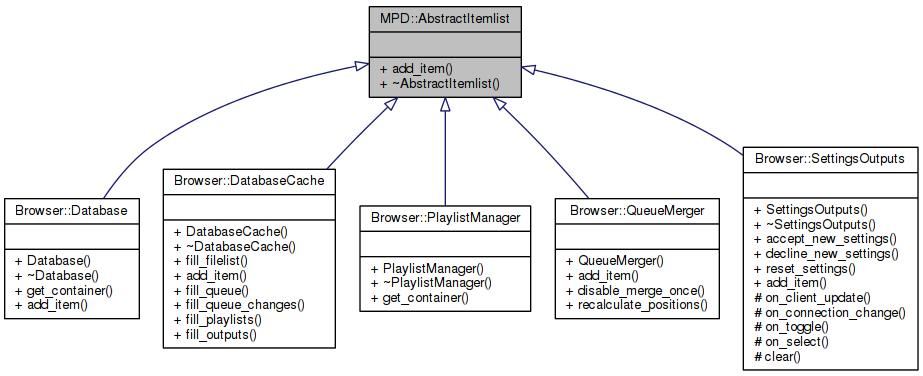
\includegraphics[width=\textwidth]{AbstractItemlist.png}
    \caption{Die AbstractItemList}
    \label{c_abstract_item_list}
\end{figure}

Für bestimmte Client Funktionen muss eine Nutzerklasse von \emph{AbstractItemlist} ableiten (siehe \ref{c_abstract_item_list}).
Leitet man ab, so muss die Methode add\_item(AbstractComposite * data) implementiert werden. 
Je nach Bedarf kann über \verb+static_cast<Zieltyp*>(data)+ der entsprechende Datentyp ,,rausgecasted'' werden.
Beim Aufruf von MPD::Client::fill\_queue ruft der Client die add\_item Methode für jeden 
Song den er vom Server bekommt auf. Die ableitende Klasse kann diese dann verarbeiten.

Dadurch werden alle Methoden von AbstractItemGenerator (bzw. die Klassen die davon ableiten) benutzbar.
%<Klassendiagramm, bzw. Klassen die es verwenden von Doxygen nehmen>

\subsubsection{AbstractItemGenerator}
%
%
%
% Hier wäre noch ein Sequenzdiagramm nötig,
% zB. für die Funktion fill_outputs( ) - beim Aufruf.

Lässt ableitende Klasse folgende Methoden implementieren:
Jede dieser Methoden ruft MPD::Playlist add\_item() von \emph{AbstractItemlist} auf um ihre Resultate weiterzugeben.
Sie erlaubt den Einsatz des \emph{Proxy-Patterns}.\footnote{http://en.wikipedia.org/wiki/Proxy\_pattern}
Andere Klassen können sich so als Client ,,ausgeben''.
Dies fand Anwendung bei der Klasse ,,DatabaseCache'' weiter unten.
\\
%<Sequenzdiagramm>   
Holt alle Songs der aktuellen Queue.
\begin{verbatim}            
    void fill_queue(AbstractItemlist& data_model);
\end{verbatim}

Holt alle geänderten Songs in der Queue seit der Version last\_version. Die Position des ersten geänderten Songs wird in first\_pos gespeichert. 
\begin{verbatim}
    void fill_queue_changes(AbstractItemlist& data_model,
                            unsigned last_version,
                            unsigned& first_pos);
\end{verbatim}

Holt alle gespeicherten Playlisten vom Server.
\begin{verbatim}              
    void fill_playlists(AbstractItemlist& data_model);
\end{verbatim}

Holt alle Audio Outputs vom Server.
\begin{verbatim}
    void fill\_outputs(AbstractItemlist& data\_model);
\end{verbatim}

Holt ein Listing aller Songs und Directories aus der Datenbank im Pfad 'path' (nicht rekursiv!)              
\begin{verbatim}
    void fill_filelist(AbstractItemlist& data_model, const char * path);
\end{verbatim}

%<Klassendiagramm, bzw. Klassen die es verwenden von Doxygen nehmen>

%-------------------------------------------
\newpage
\begin{figure}[htb!]
\subsubsection{AbstractComposite}
	\centering
        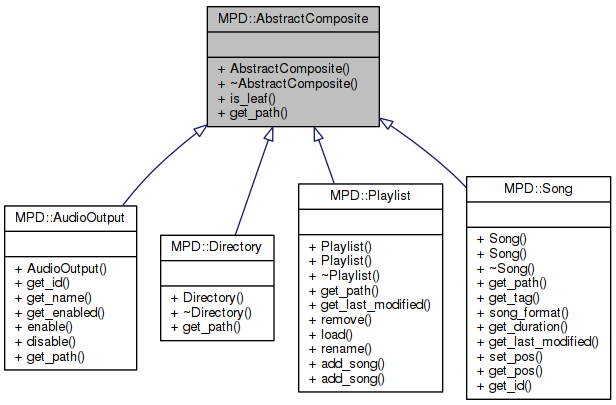
\includegraphics[width=\textwidth]{AbstractComposite.png}
	\caption{Klassendiagramm zu AbstractComposite}
	\label{c_abstract_composite}
\end{figure}

Vereinheitlicht Zugriff auf Komponenten verschiedenen Typs.
Die abstrakte Klasse (siehe Abb.: \ref{c_abstract_composite}) zwingt seine Kinder dazu eine \emph{get\_path()} Funktion zu implementieren die die Lage im virtuellen Filesystem des Servers angibt.
Der Hauptanwender dieser Klasse ist der Databasebrowser, bzw. der dahinter gelagerte Cache, da AbstractComposite es erlaubt Songs und Verzeichnisse gleich zu behandeln (vgl. Composite Pattern).
\\
Die erbende Klasse muss im Konstruktor angeben, ob es sich bei der Klasse um ein ,,File'' (\emph{true} für MPD::Song) oder um einen ,,Container'' (\emph{false} für MPD::Directory) handelt.
Diese ,,is\_leaf'' Eigenschaft kann später mit der Funktion \emph{is\_leaf()} abgefragt werden.

% <Klassendiagramm für alle Klassen die von AbstractComposite erben, siehe Doxygen>

%-------------------------------------------
\newpage
\begin{figure}[htb!]

\subsubsection{AbstractClientExtension}

	\centering
        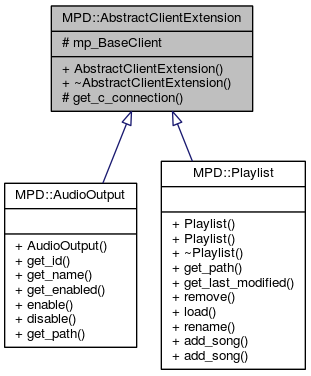
\includegraphics[scale=0.8]{AbstractClientExtension.png}
	\caption{Klassendiagramm zu AbstractClientExtension}
	\label{c_abstract_client_extension}
\end{figure}


Diese abstrakte Klasse erlaubt abgeleiteten Klassen ähnlich zum BaseClient eigene Kommandos zu implementieren (siehe \ref{c_abstract_client_extension}).
Dies geschieht indem die abstrakte Klasse eine Referenz auf den BaseClient im Konstruktor erwartet und speichert.
Ableitende Klassen können die \textit{protected} get\_c\_connection() Methode benutzen um eigene Kommandos zu implementieren.

\begin{verbatim}
   AbstractClientExtension(MPD::BaseClient& base_client)
\end{verbatim}

\emph{AbstractClientExtension} wird in diesem Entwurf von MPD::Playlist und MPD::AudioOutput benutzt.
Man kann allerdings darüber diskutieren dass dieses abstrakte Klasse der Modelschicht die Möglichkeit gibt zu ausgefeilte Logik zu implementieren, was nach dem MVC Paradigma nicht sein sollte.  
Da die Logik meist darin besteht einfache Kommandos an den Server zu schicken, wurde dieser Weg gewählt um 
den Entwurf zu vereinfachen.


%=============================================


\newpage
\begin{figure}[thb!]
\subsubsection{Namespace-Übersicht}
    \centering
    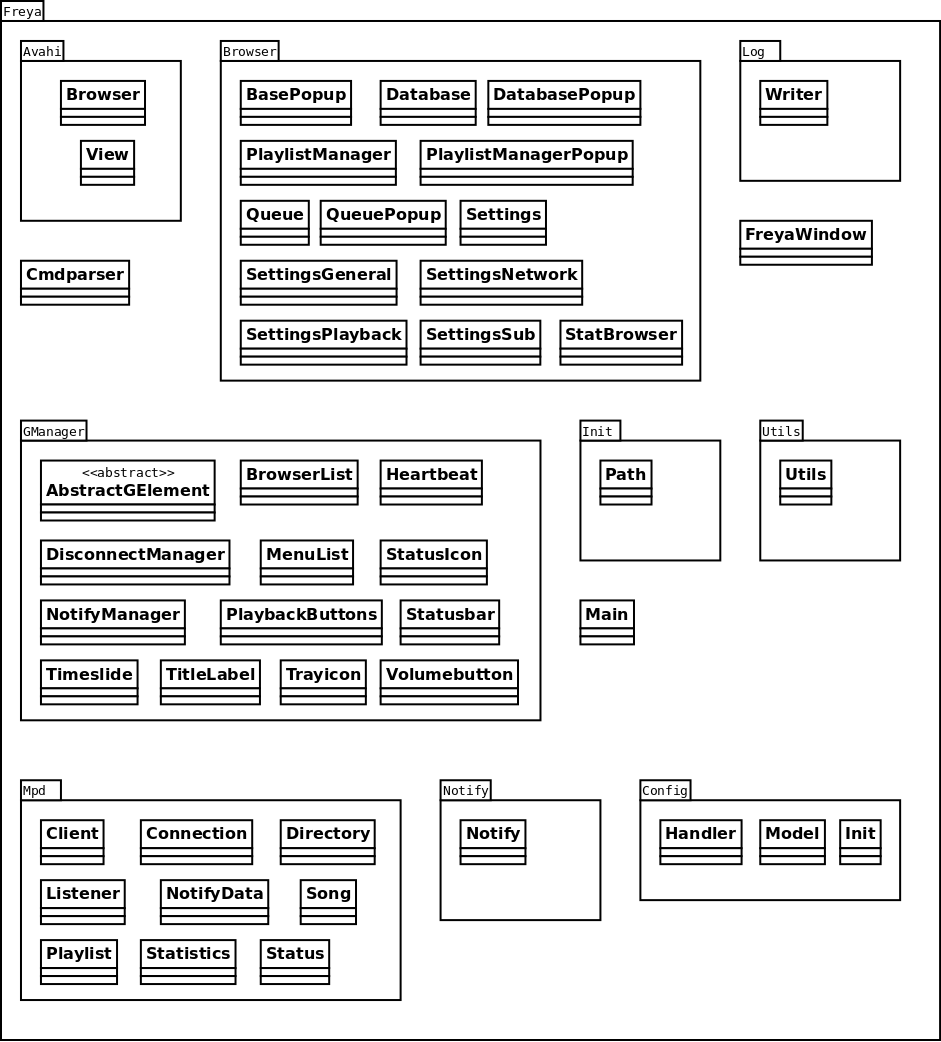
\includegraphics[scale=0.50]{Namespace_Uebersicht.png}
    \caption{Die Namespaces im Überblick}
    \label{dd_namespaces}
\end{figure}

\section{Utils und Writer} 

\subsection{Utils}
Im \emph{Utils Namespace} sollen sollen sich folgende Hilfsfunktionen zur Zeit/Datumsumrechnung befinden:

\begin{itemize}
    \item Umrechnung von Sekunden in einen ,,Dauer-String Bsp'' : ,,4 hours 2 minutes 0 seconds''

        \begin{verbatim}
        Glib::ustring seconds_to_duration(unsigned long);
        \end{verbatim}

    \item Umrechnung Sekunden in einen Timestamp, Bsp: ,,2011-04-02''
        \begin{verbatim}
        Glib::ustring seconds_to_timestamp(const long);
        \end{verbatim}

    \item Umwandlung eines Integer Wertes in einen String
        \begin{verbatim}
        std::string int_to_string(int num);
        \end{verbatim}
\end{itemize}


Diese grundlegenden Funktionen sollen ausgelagert werden damit sie von mehreren Klassen verwendet werden können und um Redundanzen im 
Code zu vermeiden.

\subsection{Logging}

Im \emph{Log Namespace} befindet sich die Writer Klasse, welche auch als sog. ,,\textit{Utils-Klasse}'' Funktionen für alle anderen
Klassen in Namespace bereitstellt. Bei dieser Klasse wurde das Singleton Pattern gewählt, damit sie ,,leicht von überall'' aus erreichbar ist, ohne dass vorher explizit eine Instanzierung statt finden muss. Die Logdatei wird im Konfigurationsverzeichnis von Freya als log.txt
abgespeichert, im folgenden Dokument gibts dazu mehr Informationen. 
Die Logklasse dient zur Protokollierung von Fehlern und besonderen Ereignissen.  

\begin{figure}[htb!]
    Folgende selbsterklärende Makros werden von der \emph{Log::Writer} Klasse zur Protokollierung bereitgestellt:

    \begin{verbatim}
    Warning(msg, ...)  _MSG(Log::LOG_WARN, msg, ##__VA_ARGS__)
    Info(msg, ...)     _MSG(Log::LOG_INFO, msg, ##__VA_ARGS__)
    Fatal(msg, ...)    _MSG(Log::LOG_FATAL_ERROR, msg, ##__VA_ARGS__)
    Error(msg, ...)    _MSG(Log::LOG_ERROR, msg, ##__VA_ARGS__)
    Debug(msg, ...)    _MSG(Log::LOG_DEBUG, msg, ##__VA_ARGS__)
    Success(msg, ...)  _MSG(Log::LOG_OK, msg, ##__VA_ARGS__)
    \end{verbatim}
\end{figure}

%----------------------------------------------------------------------------------------------

\section{Config Hauptklassen}

\subsection{Path}
Die \emph{Init::Path} Klasse soll für die Initialisierung und das Management der Freya Config Pfade zuständig sein.
Bei der Initialisierung soll überprüft werden ob das Konfigurationsverzeichnis vorhanden ist, wenn nicht wird ein Neues
angelegt und anschließend wird eine default config.xml geschrieben. Eine Standardkonfiguration ist im Quellcode als 
konstanter globaler String einkompiliert.
\\
\\
Schlägt das Erstellen der Konfigurationsdatei fehl, so soll versucht werden eine entsprechende Fehlermeldung in die Log Datei zu schreiben, 
falls diese zuvor erfolgreich angelegt wurde. Zusätzlich sollen DEBUG Ausgaben auf dem Bildschirm angezeigt werden, wenn das Programm
über ein Terminal gestartet wird.

\paragraph{Instanzierung der Path Klasse kurz erläutert:}
Bei der Instanzierung werden die private Methoden get\_config\_dir() und get\_config\_path() aufgerufen, deren Rückgabewerte werden
als Membervariablen der Init::Path gespeichert. Diese Methoden nutzen die g\_get\_user\_config\_dir() glib Methode
welche den User Pfad nach XDG Standard zurückliefert.\footnote{http://standards.freedesktop.org/basedir-spec/basedir-spec-latest.html}
\\
\\
Je nach Funktion, wird an den Pfad ein ,,/freya'' für das Freya Konfigurationsverzeichnis, ,,config.xml''
für die Konfigurationsdatei oder ,,log.txt'' für die Logdatei dran gehängt.
\\
\\
Bei der Initialisierung wird die dir\_is\_avaiable()
Methode aufgerufen. Diese prüft ob die nötigen Verzeichnisse und Dateien existieren, wenn nicht wird versucht diese
anzulegen. Diese Klasse schreibt DEBUG und ERROR Ausgaben auf die Konsole raus, da zum Zeitpunkt der Initialisierung
nicht gewährleistet werden kann dass eine Logdatei existiert.


\paragraph{Die ,,dir is available()'' Methode kurz erläutert:}
Diese Methode prüft zuerst über die glib Funktione g\_file\_test() ob ein ,,freya'' Verzeichnis existiert,
ist dies nicht der Fall werden die privaten Methoden create\_dir() und create\_config() aufgerufen.
Ist ein ,,freya'' Verzeichnis vorhanden, so wird über die glib g\_file\_test() Funktion geprüft ob die Konfigurationsdatei
config.xml existiert. Existiert diese nicht, so wird die private create\_config Methode() aufgerufen.
Existiert diese, so wird mittels der glib g\_access() Methode geschaut ob diese lesbar und beschreibar ist. 
Bei Misserfolg wird über die glib Funktion g\_warning eine entsprechende Fehlermeldung auf
dem Bildschirm (Konsole) ausgegeben, da die Logklasse zu diesem Zeitpunkt noch nicht aufgebaut worden ist.


\paragraph{Die ,,create config()'' Methode kurz erläutert:}
Die Mothode soll zum Anlegen eines Konfigurationsverzeichnisses verwendet werden.
Im Fehlerfall wird eine entsprechende Warnung über glib Funktion g\_warning() auf dem Bildschirm ausgegeben.

\paragraph{Die ,,create dir()'' Methode erläutert:}
Diese Methode bietet die Funktionalität über die glib Funktion g\_mkdir\_with\_parents(configdir,0755) ein Verzeichnis mit den rechten 755 (drwxr-r-xr-x) anzulegen. Bei Erfolg wird mit g\_message() eine Erfolgsmeldung auf dem Bildschirm (Konsole)
ausgegeben, andernfalls eine warnung mit g\_warning().


%----------------------------------------------------------------------------------------------

\subsection{Konfigurationsdatei}

Die Freya Konfigurationsdatei soll im simplen XML Format realisiert werden, XML wird gewählt um das Parsen zu vereinfachen und um
ein standardisiertes Format nach außen bereitzustellen. 
\\
Die Konfigurations- und Logdatei soll nach XDG Standard \verb+($XDG_CONFIG_HOME)+ unter \verb+$HOME/.config/freya/<config.xml,log.txt>+ gespeichert werden.

\begin{itemize}
    \item \url{http://standards.freedesktop.org/basedir-spec/basedir-spec-latest.html#variables}
\end{itemize}

Die Optionen in der Konfigurationsdatei sind baumartig nach ,,Domainprinzip'' aufgebaut. Die Konfigurationsdatei unter \ref{c_config}
zeigt exemplarisch den gewünschten Aufbau.

\begin{figure}[htb!]
    \lstinputlisting[language=XML]{config.xml}
    \caption{Config.xml Konfigurationsdatei im Überblick}
    \label{c_config}
\end{figure}


\subsection{Model}
Die \emph{Config::Model} Klasse gehört nach dem MVC Paradigma zur Model Schicht. Diese Klasse soll die nötigen Daten (Konfigurationsdatei)
die zum Betrieb von Freya nötig sind im Speicher vorhalten und Methoden zum Lesen und Speichern der Konfigurationsdatei auf die Festplatte bereit stellen (siehe \ref{c_confmod}).

\begin{figure}[htb!]
    \centering
    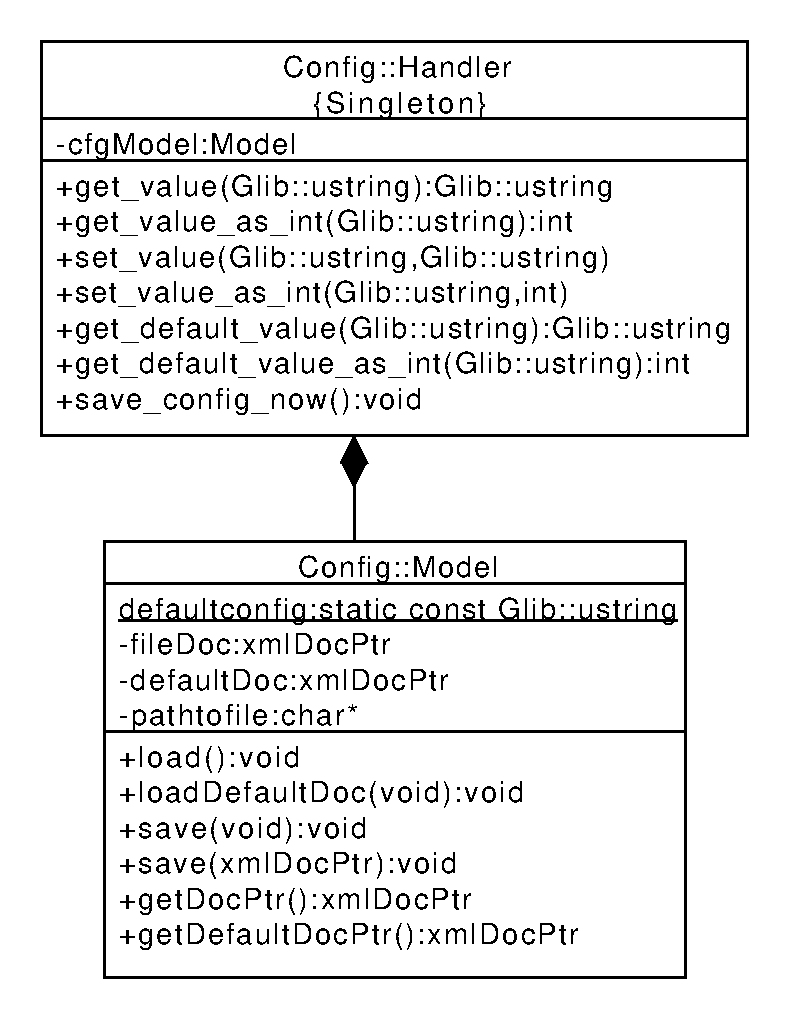
\includegraphics[scale=0.6]{configClass.pdf}
    \caption{Config-Model Beziechung}
    \label{c_confmod}
\end{figure}


Zum Parsen der XML Datei soll hier die C Programmbibliothek libxml2 verwendet werden. Diese Library wurde gewählt, weil sie alle benötigten Funktionen enthält, nach dem ANSI-C Standard implementiert ist
und bereits seit über einem Jahrzehnt Quasi-Standard im C Umfeld ist.

Informationen zur zu verwendenden Libaray:

    \begin{itemize}
        \item \url{http://xmlsoft.org/}
        \item \url{http://en.wikipedia.org/wiki/Libxml2}
    \end{itemize}

\begin{figure}[htb!]
    \centering
    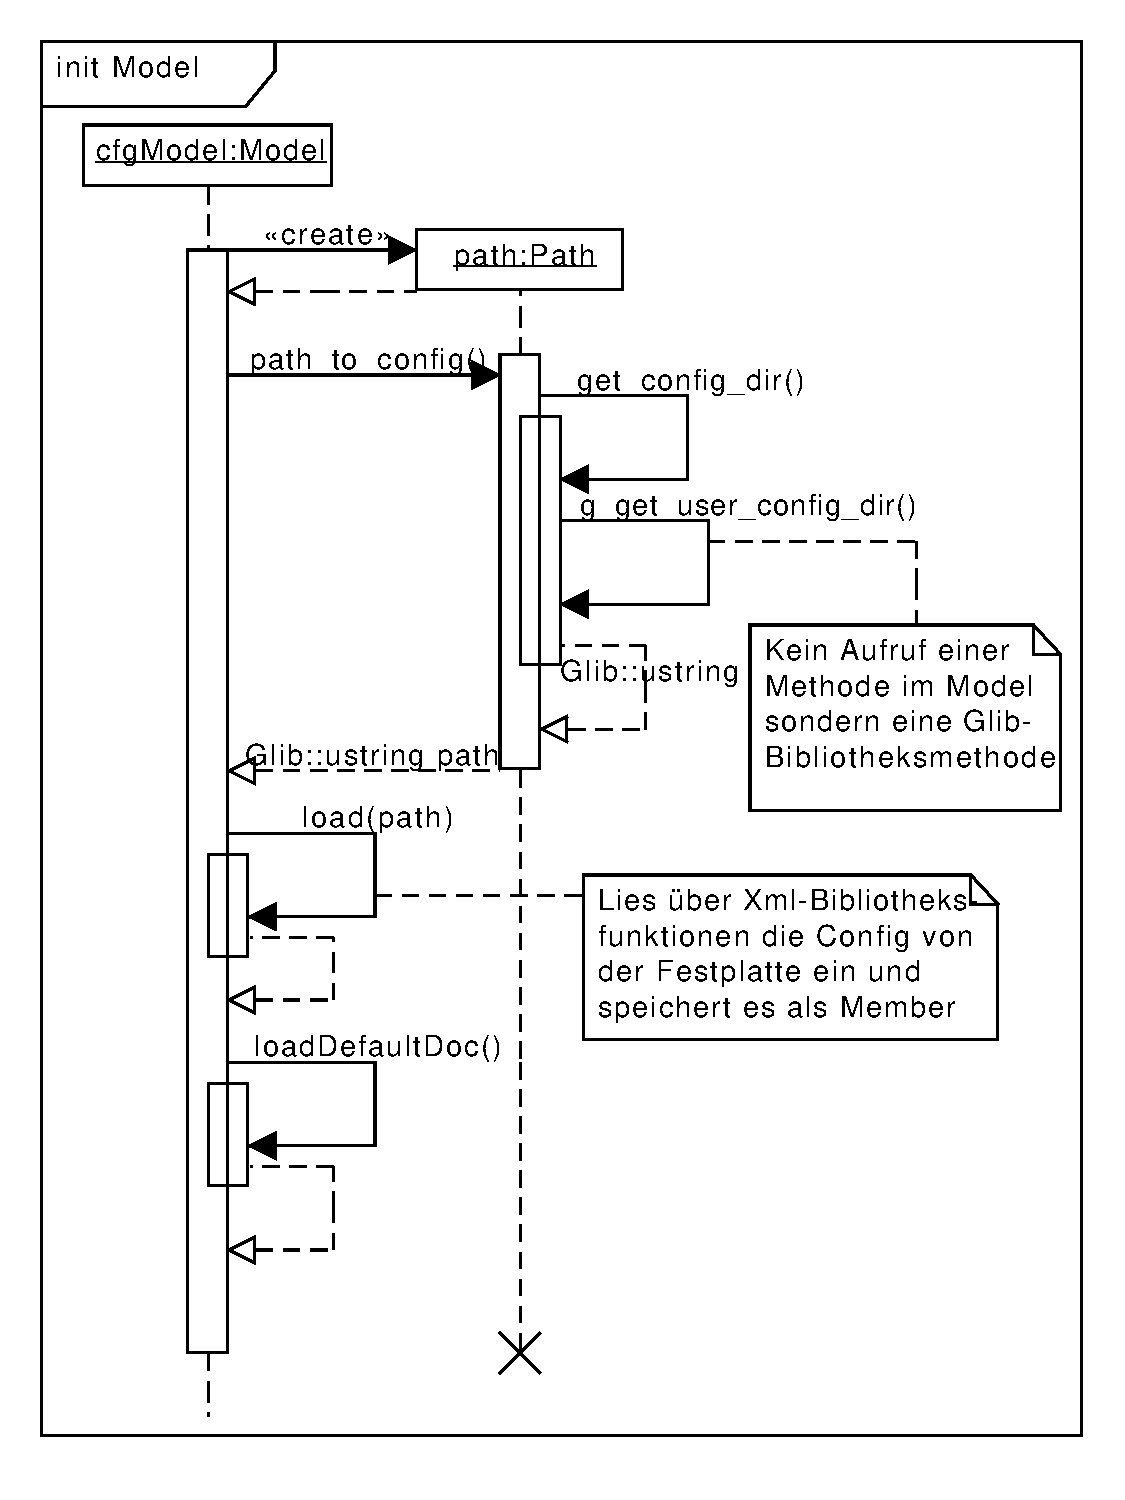
\includegraphics[scale=0.6]{init.pdf}
    \caption{Initialisierung des Models}
    \label{c_modelinit}
\end{figure}


\subsubsection{Instanzierung des Models}


Über die \emph{Init::Path} Klasse holt sich das Model bei seiner Instanziierung über die path\_to\_config() Methode
den Pfad zur Konfigurationsdatei, parst diese sowie die einkompilierte default Config und 
initialisiert zwei XML Document Pointer die auf ein DOM Objekt, welches einen Dokumentenbaum enthält, zeigen.
Hierzu werden die privaten load(pathtofile) und die loadDefaulDoc() Methoden der Config::Model Klasse verwendet.
\\   

Anschließend kann man über diese DOM Objekte traversieren und Werte der Konfigurationsdatei lesen oder setzten.
Die default config wurde implementiert um fehlerhaften Werten oder einer kaputten Konfiguration vorzubeugen. Ist ein benötigter Wert
nicht in der User config vorhanden oder ist diese beschädigt so wird auf die default config zurückgegriffen.
Bei Beendigung des Models wird das aktuelle Objekt als XML Konfigurationsdatei auf die Festplatte geschrieben.
Wie andere Objekte auch, nutzt das Model die Log-Klasse um zu Informationen und Fehler zu protokollieren.



\subsubsection{Prinzipieller Ablauf der load() Methode}

Beim Instanzieren ruft das Model seine load() Methode mit dem aktuellem Pfad auf.
In dieser wird als Erstes die libxml2 Methode xmlParseFile(pathtofile) aufgerufen. Diese bekommt den
Pfad zur Konfigurationsdatei übergeben und versucht über den übergebenen Pfad das File zu laden.
\\
Wenn die Operation erfolgareich war, wird ein Dokument Pointer von der xmlParseFile() 
zurückgegben, im Fehlerfall wird \emph{NULL} zurückgegeben.
\\
Anschließend wird das geladene Dokument auf Gültigkeit geprüft, zeigt dieses auf \emph{NULL} so wird eine entsprechende Fehlermeldung über den Log::Writer in die Logdatei geschreiben. Wurde ein gültiger xmlDocPtr zurückgegeben so soll folgendes passieren:

\begin{itemize}
    \item Ein Node Pointer wird auf das root Element über xmlDocGetRootElement() gesetzt
    \item Überprüfung ob Node Pointer Null ist, trifft das zu, so wird ein Error in die Logdatei geschrieben
        allokierter Speicher vom Dokument Pointer mittels xmlFreeDoc() freigegeben und dieser auf NULL gesetzet
    \item Ist der Node Pointer gültig, so wird mittels der libxml2 Methode xmlStrcmp(DocPtr, ,,freya'') geprüft ob das
        root Element ,,freya'' entspricht. Ist dies der Fall wird eine Erfolgsmeldung in die Logdatei geschreiben. Im Fehlerfall wird eine Fehlermeldung rausgeschreiben, allokierter Speicher freigegeben
        und der Dokument sowie der Node Pointer auf \emph{NULL} gesetzt. 
\end{itemize}


\subsubsection{loadDefaultDoc() Methode}
Diese Methode holt sich die default Konfigurationsdatei aus einem einkompilierten String.
Dieser String wird anschließend mittels der libxml2 xmlParseMemory() geparst und ein xmlDocPtr zurückgegeben welcher als defaultDoc Membervariable gespeichert wird.

\subsubsection{Ablauf der save() Methode}
Die save() Methode ist eine Wrapper Methode für save(char*, xmlDocPtr). Sie ruft lediglich diese mit dem aktuellen Dokument Pointer und dem Pfad zur config.xml auf.

\begin{figure}[htb!]
    Quellen zur Implementierung:
    \begin{itemize}
        \item \url{http://xmlsoft.org/tutorial/index.html}
        \item \url{http://student.santarosa.edu/~dturover/?node=libxml2}
    \end{itemize}
\end{figure}



\subsection{Handler}
Die Config::Handler Klasse gehört nach dem MVC Paradigma zur Controller Schicht. Diese Klasse soll für das Management bzw für den
Zugriff auf das Model und somit die Konfigurationsdatei zuständig sein. Sie enthält Methoden zum Lesen und Setzen der einzelnen Optionen.
\\
\\
Der Config::Handler wird als Singleton implementiert um einen zentralen Zugriff für alle anderen Programmteile über eine einzelne Schnittstelle zu ermöglichen.
\\
\\
Der Handler soll einen Pointer als Membervariable auf das aktuelle Model Objekt bekommen um direkten Zugriff auf die Dokument Pointer
zu haben. Desweiteren sollen Wrapper um die get und set value Methoden geschrieben werden um verschiedene Datentypen lesen und setzen zu können, so kann gleich eine ,,Teilvalidierung'' erfolgen.

\begin{figure}[htb!]
    Der Config::Handler stellt folgende Makros bereit:
    \begin{verbatim}
    CONFIG_SET(x,y) 
    CONFIG_GET(x)   
    CONFIG_SET_AS_INT(x,y) 
    CONFIG_GET_AS_INT(x)   
    CONFIG_SAVE_NOW() 
    CONFIG_GET_DEFAULT(x)
    CONFIG_GET_DEFAULT_AS_INT(x)
    \end{verbatim}
\end{figure}

\begin{figure}[htb!]
Über die \emph{save\_now()} Abb. \ref{c_configsave} Methode soll die aktuelle Konfiguration direkt über das Model gespeichert werden können.
Alle Methoden nutzen nach Möglichkeit Log::Writer um Informationen und Fehler in der Logdatei zu protokollieren.


    \centering
    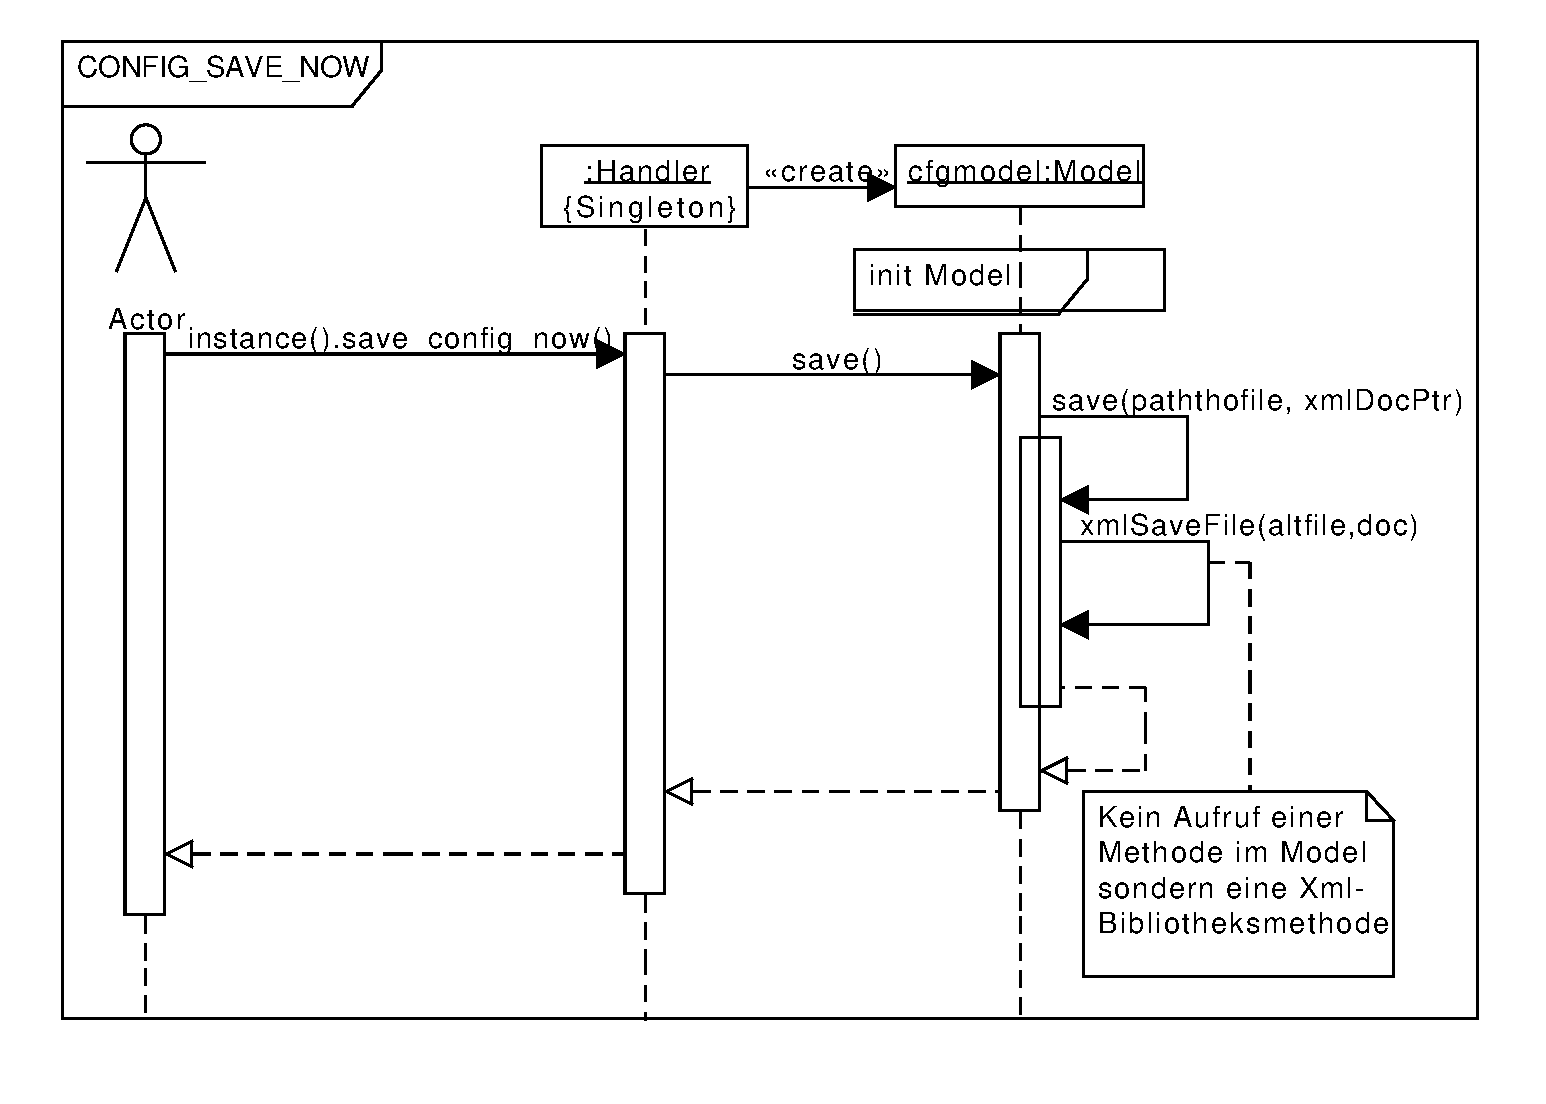
\includegraphics[width=\textwidth]{configSave.pdf}
    \caption{Ablauf der Config Save Methode}
    \label{c_configsave}
\end{figure}

\begin{figure}[htb!]
    \centering
    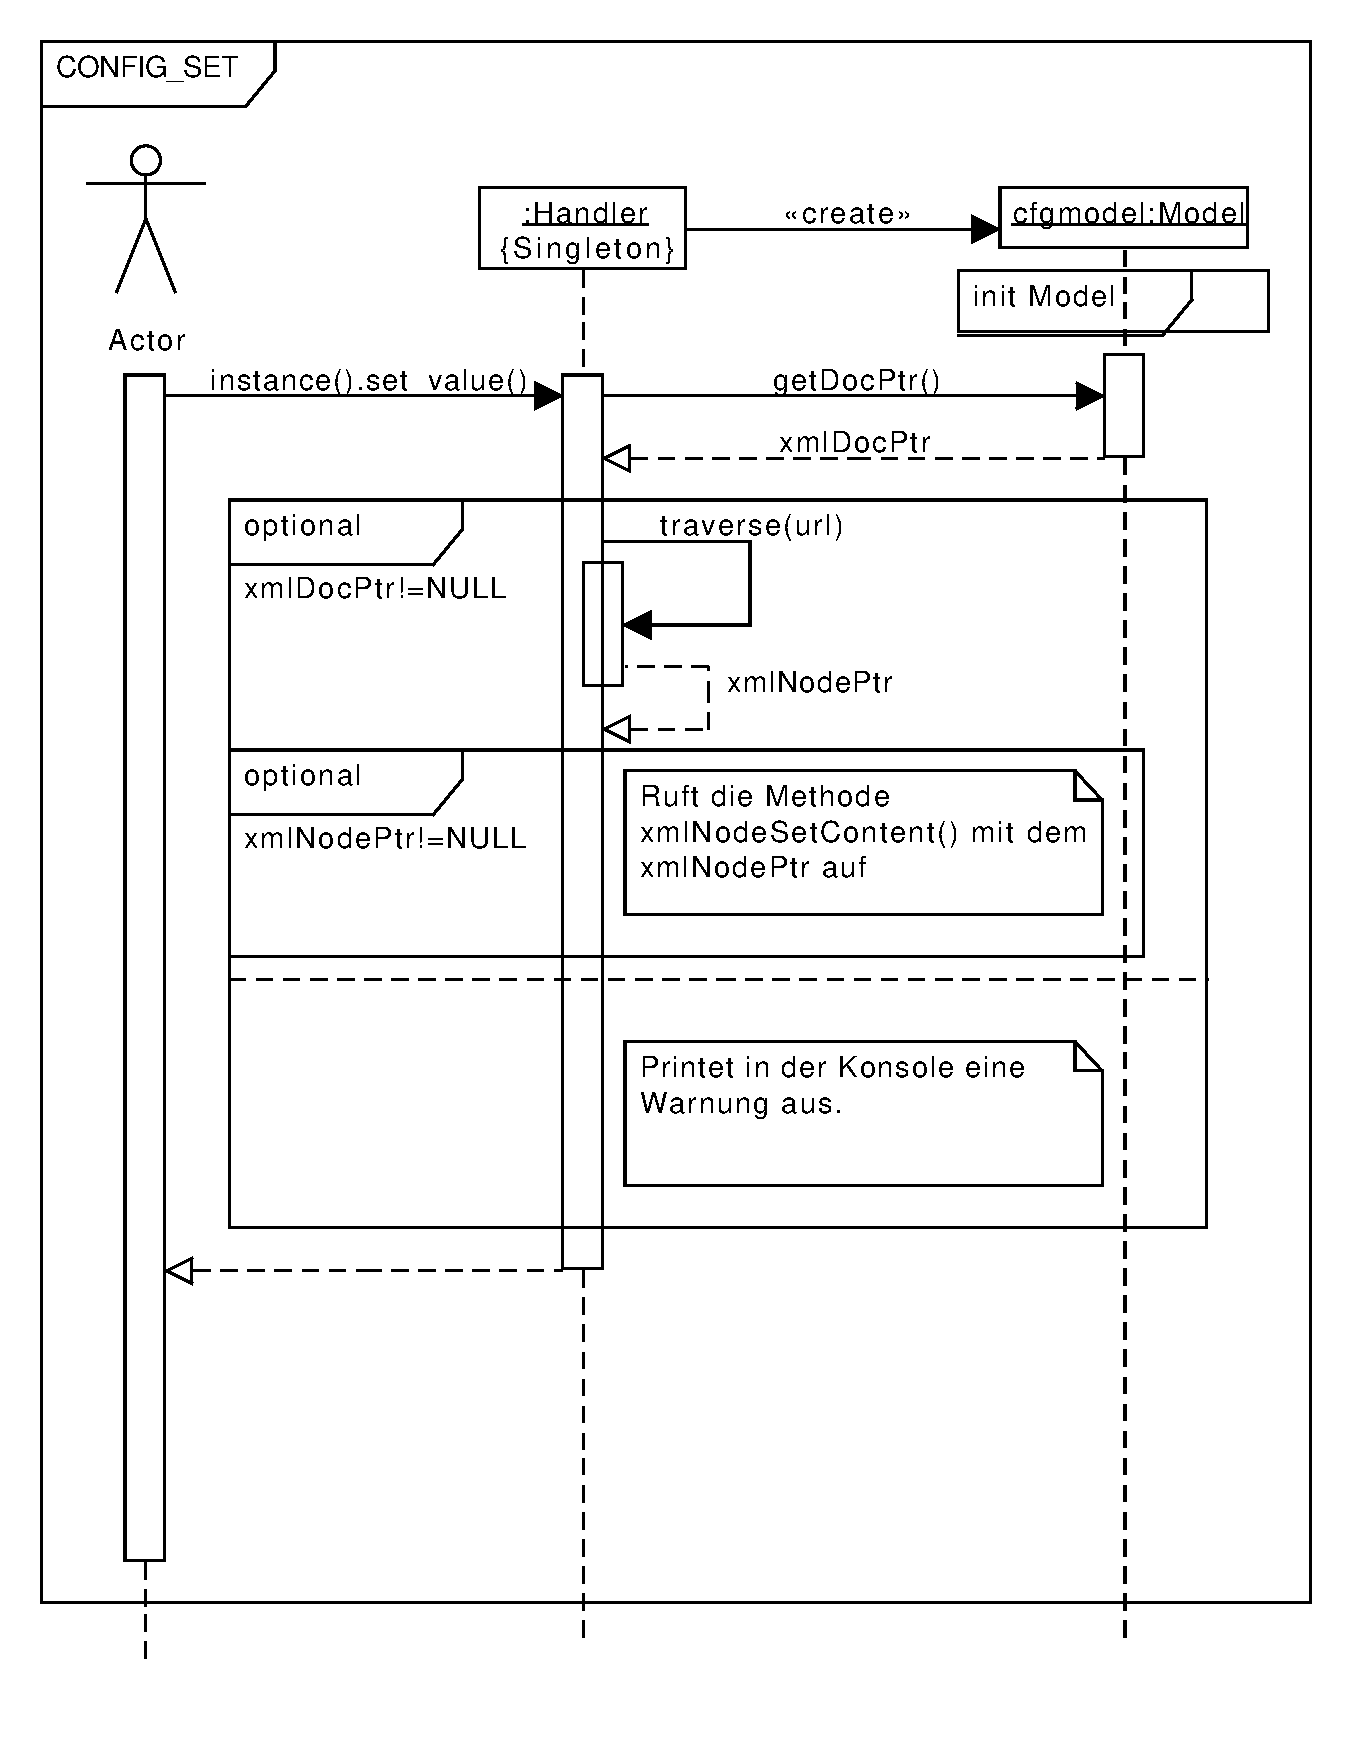
\includegraphics[scale=0.5]{configset.pdf}
    \caption{Config get vlaue() Ablauf}
    \label{c_configget}
\end{figure}

\newpage
\paragraph{Grober Ablauf beim setzen einer Integer Wertes:}

\begin{itemize}

    \item Aufruf des \verb+CONFIG_SET_AS_INT("settings.connection.port",6667)+ Makros
    \item Über das Makro wird die Wrapper Methode \verb+set_value_as_int()+ aufgerufen
    \item Diese Methode wandelt den Integer Wert in einen String um und ruft die eigentliche set Methode set\_value(url, wert) auf
    \item Die set\_value(url, wert) Methode holt sich mit cfgmodel.getDocPtr() einen aktuellen Dokument Pointer über das Model
    \item Ist der Dokument Pointer \emph{NULL}, so kann kein Wert geschrieben werden, also wird über den Log:Writer
        eine entsprechende Warnung in die Logdatei geschreiben.
    \item Bei einem gültigem Dokument Pointer wird  mittels xmlDocGetRootElement() auf das root Element zugegriffen
    \item Anschließend wird mit xmlChildrenNode der Node Pointer auf den folgenden Kinderknoden gesetzt und die traverse() Methode aufgerufen
    \item Nun werden diverse Vorbereitungen getätigt und anschließend rekursiv im Baum nach der übergebenen
        Url gesucht. Hierbei wird jeweils der rekursive Teilstring (eins.zwei.drei) gemäß dem Url Aufbau untersucht

    \item Wird die Url nicht gefunden oder sind andere Fehler aufgetreten wird ein \emph{NULL Pointer} zurückgegeben und eine entsprechende Fehlermeldung in die Logdatei geschrieben
    \item Wird die Url gefunden, so wird ein NodePointer auf den Optionswert über die Aufruferkette an die set\_value() Methode \emph{returned}. In dieser wird dann der Wert an der entsprechende Stelle gesetzt.  
\end{itemize}


\begin{figure}[htb!]
    \centering
    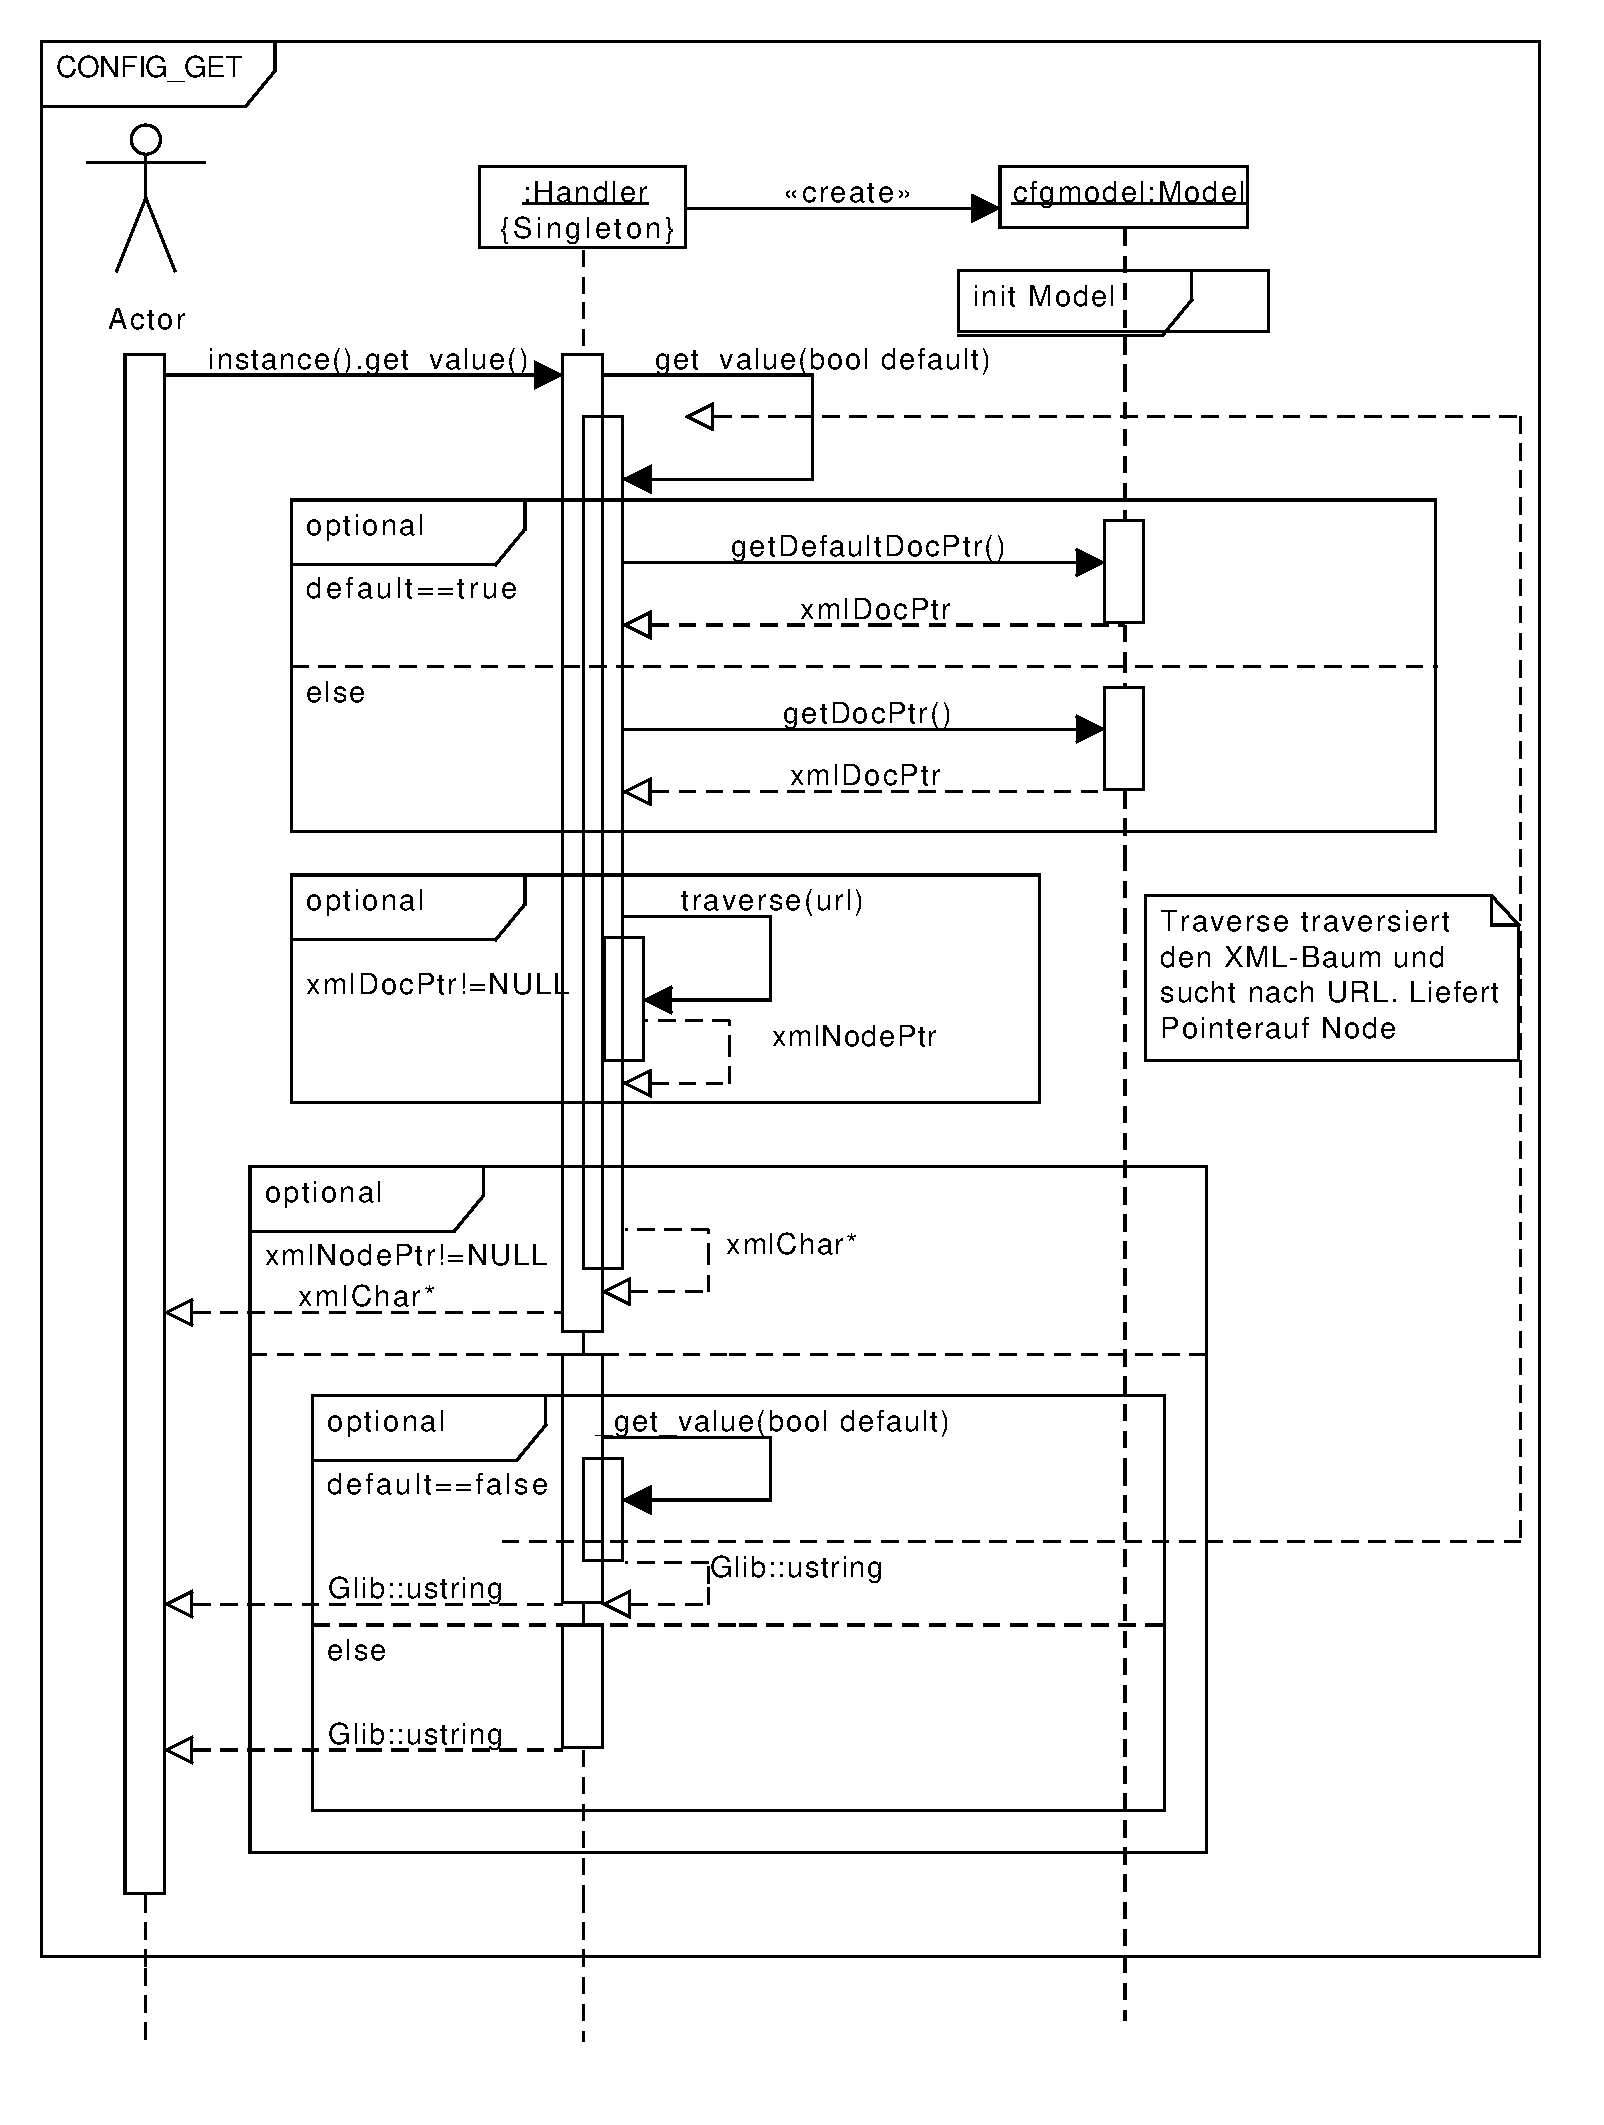
\includegraphics[scale=0.5]{configget.pdf}
    \caption{Config get\_value() Ablauf}
    \label{c_configget}
\end{figure}

%-------------------------------------------


\paragraph{Grober Ablauf beim Lesen eines Wertes:}

\begin{itemize}
    \item Das Makro \verb+CONFIG_GET("settings.connection.host")+ wird analog dem Setzen aufgerufen, dieses ruft die entsprechende Wrapper
        Methode get\_value() welche die eigentliche private \_get\_value() Methode aufruft.
        \\
        Der zweite Parameter dieser Methode ist ein \emph{boolean flag}, dieser dient dazu der \_get\_value()
        Methode mitzuteilen ob der entsprechende Default Wert Pointer, welcher auf die einkompilierte
        Konfigurationsdatei zeigt, oder der Custom User Config Pointer geladen werden soll.
    \item Die \_get\_value() Methode holt entsprechend dem flag, den ,,richtigen'' Dokument Pointer über das Model (analog Setzen eines Integer Wertes)
    \item Bei einen gültigen Pointer wird analog zum Setzen der Node Pointer auf das erste Element gesetzt und \textit{traverse()}
        aufgerufen (siehe Setzen eines Wertes).
    \item Kann kein Node ermittelt werden (d.h. cur Pointer zeigte auf NULL nach dem traversieren), so wird eine entsprechende Warnung in die Logdatei geschreiben.
    \item Anschließend wird die \_get\_value(url,true) Methode rekursiv mit einem \emph{true flag} aufgerufen. Aufgrund des true flags wird nun der Dokument Pointer mit den Default Werten geladen.
    \item Analog zum bisherigen Verlauf beim ,,Lesen eines Wertes'' erfolgt die Suche des Default Wertes. Kann am Ende kein
        Default Wert ermittelt werden so wird an den Aufrufer eine leerer String zurückgegeben.
\end{itemize}











\section{GUI Elementklassen}
\subsection{Interaktion des Clients mit anderen Modulen}
\begin{itemize}
\item Die meisten GUI Klassen leiten von \emph{AbstractClientUser} ab und speichern daher eine Referenz auf eine Instanz von \emph{MPD::Client}
      Sie können daher Funktionen wie queue\_add() direkt aufrufen.
      AbstractClientUser zwingt die abgeleitenden Klassen folgende Funktionen zu implementieren: 
\begin{verbatim} 
   1) void on_client_update(mpd_idle event, MPD::NotifyData& data)
   2) void on_connection_change(bool server_changed, bool is_connected)
\end{verbatim}
   \begin{enumerate}
   \item Wird aufgerufen sobald der Listener ein Event festgestellt hat. Für jedes eingetretene Event wird on\_client\_update()    
   einmal aufgerufen. ,,event'' ist dabei eine Enumeration aller möglichen Events, die von libmpdclient 
   vorgegeben werden. (Siehe auch \url{http://www.musicpd.org/doc/libmpdclient/idle\_8h.html#a3378f7a24c714d7cb1058232330d7a1c})
   ,,data'' ist eine Referenz auf eine Instanz von MPD::NotifyData. Die benutzenden Klassen können folgenden Funktionen so
   bei Events sofort die aktuellen Änderungen auslesen:
   \begin{itemize} 
     \item get\_status() gibt den aktuellen MPD::Status
     \item get\_song() gibt den aktuellen MPD::Song
     \item get\_statistics() gibt die aktuellen MPD::Statistics
   \end{itemize} 
   \item Wird vom Client aufgerufen sobald die Verbindung verloren geht.
         Dabei zeigt der übergebene boolean Wert ,,is\_connected'' an ob man connected oder disconnected wurde.
         ,,server\_changed'' soll dann anzeigen ob der Server derselbe ist wie beim zuvor geschehenen Connectvorgang.
         Dies ist beim ersten Start stets wahr. ,,server\_changed'' kann nicht wahr sein wenn ,,is\_connected'' falsch ist.
   \end{enumerate}
\item Ableitung von den oben beschriebenen abstrakten Klassen AbstractItemlist und AbstractFilebrowser, um alle Funktionen von AbstractItemGenerator nutzen zu können. Beispiele dazu folgen weiter unten.
\end{itemize}


\subsection{Hauptklassen}
Der GManager Namespace enthält Klassen die der Verwaltung und Kontrolle des Hauptfensters von Freya dienen,
jedoch nicht den eigentlichen Inhalt des Hauptfensters bereitstellen (dies soll von den Browserklassen getan werden)
Alle Klassen gehören nach dem MVC Paradigma der Controllerschicht an.
\\
Der Begriff ,,Browser'' wird im folgenden für die einzelnen Tabs benutzt die Links in der Sidebar zu finden sind. 
Beispiele dafür sind ,,Queue'', ,,Database'' und ,,Settings''.
\\
Viele Klassen sind nur stichpunktartig erklärt da sie oft einander ähnlich sind, und ein gewisser Freiraum bei der Implementierung der
GUI gelassen werden soll.


\subsubsection{AbstractBrowser}
Eine abstrakte Basisklasse durch die...
\begin{verbatim}
  Gtk::Widget * get_container(void) 
\end{verbatim}
..implementiert werden muss. Diese sollte den umliegenden Container des Browser als Pointer zurückgeben,
so dass \textit{GManager::BrowserList} diesen (und damit seine Kinder) im Hauptbereich anzeigen kann.
Siehe auch GManager::BrowserList für die nähere Erklärung zu den anderen nicht-abstrakten Methoden dieser Klasse.

\subsubsection{BrowserList}
Zeigt eine Liste von Browsern in der Sidebar.
\begin{itemize} 
\item Bietet eine add() Methode die eine Referenz auf AbstractBrowser erwartet und fügt diesen Browser in der Sidebar hinzu.
\item set() zeigt den Browser im Hauptbereich, ohne ihn hinzuzufügen.
\end{itemize}
Die Klasse benutzt alle Methoden von AbstractBrowser um diesen entsprechend anzuzeigen:
\\
Der Container der im Hauptbereich beim Wechseln angezeigt wird
\begin{verbatim}
  Gtk::Widget * get_container();
\end{verbatim}
Welcher Name soll in der Sidebar angezeigt werden?
\begin{verbatim}
  Glib::ustring get_name();
\end{verbatim}
Welche Gtk::Stock::ID (eine ID die ein Icon repräsentiert) soll in der Liste angezeigt werden?
\begin{verbatim}
  Gtk::Stock::ID get_icon_stock_id();
\end{verbatim} 
Ist sichtbar in der Leiste?
\begin{verbatim}
  bool is_visible(); 
\end{verbatim}
Benötigt dieser Browser eine Verbindung zum funktionieren?
\begin{verbatim}
  bool needs_connection(); 
\end{verbatim}

Als \emph{View} wird ein Gtk::TreeView benutzt, die Browserreferenzen werden in einem Gtk::ListStore gespeichert,
was damit das Model darstellt. 

\subsubsection{Heartbeat}
Diese Klasse soll alle 500ms ein Signal aussenden, die bisher vergangene Zeit summieren, und sich regelmäßig mit dem 
Client synchronisieren, so dass die summierte Zeit der aktuellen Zeit innerhalb des aktuellen Songs entspricht.
Über signal\_client\_update() können sich andere Klassen als Klienten registrieren:
\begin{verbatim}
  Heartbeat.signal_client_update().connect(<funktionspointer>);
\end{verbatim}
Der angegebene Funktionspointer wird dann aufgerufen und muss folgender Signatur entsprechen:
\begin{verbatim}
  void func(double time)
  {
      ...
  }
\end{verbatim}

Der übergebene Parameter ist die Zeit, die seit dem Instanzieren vergangen ist. 
Sie kann durch folgende Funktionen verändert werden:
\begin{verbatim}
void pause(void)  - Setzt das Zählen aus
void play(void)   - Fängt damit wieder an
void reset(void)  - Fängt von 0 wieder an
void get(void)    - Bekommt die jetzige Zeit
void set(void)    - Setzt die jetzige Zeit absolut und zählt von dort weiter
\end{verbatim}

Zusätzlich stoppt die Heartbeat Klasse das Zählen wenn der Client das playback pausiert.
Wird es fortgesetzt, so wird play() aufgerufen. 
Zusätzlich wird bei jedem ,,Client Event'' der Zähler an der vergangen Zeit, im gerade spielenden Song, justiert.

\subsubsection{MenuList}
Kontrolliert und verwaltet die Anzeige (Sensitivität) und Steuerung der Menüleiste.

\subsubsection{NotifyManager}
Kontrolliert und verwaltet die Anzeige von Notifications bei entsprechenden ,,events''.
Greift dabei auf die Notifylib zurück.

\subsubsection{PlaybackButtons}
Kontrolliert die Anzeige der oberen rechten ,,Playbackbuttons'' Stop, Play/Pause, Next, Previous
Das Icon des Playbuttons wird entsprechend geändert falls das Playback pausiert ist,
bzw. fortgesetzt wird. Es sollen die Buttons \it Stop, Play/Pause, Previous und Next \rm angezeigt wird.

\subsubsection{Statusbar}
Kontrolliert die Anzeige der Statusbar (was den Text miteinfasst). 
Benutzt GManager::Heartbeat um die Zeitanzeige zu aktualisieren. Ansonsten bekommt es alle Informationen rein vom Client update.

\subsubsection{StatusIcons}
Kontrolliert und verwaltet Anzeige der Icons unter der Sidebar.
Bei Aktivierung sollen die Icons eingedrückt sein.
Folgende Icons sollen dargestellt werden:
\begin{itemize}
\item Repeat-Mode (Wiederholt Queue)
\item Consume-Mode (Entfernt Song nach Abspielen aus der Queue)
\item Random-Mode (Zufälliges Abspielen innerhalb der Queue)
\item Single-Mode (Hält nach Abspielen eines Songs an)
\end{itemize}

\subsubsection{Timeslider}
Zeigt und kontrolliert die aktuelle Zeit innerhalb des momentan spielenden Liedes.
Beim Klicken innerhalb der Timeline wird zur entsprechenden Stelle im Song gesprungen.
Benutzt GManager::Heartbeat um die Zeitanzeige zu aktualisieren.

\subsubsection{TitleLabel}
Verwaltet und kontrolliert Anzeige des Titels bzw. Künstlers und Albums in der Titelleiste sowie der ,,Next Song'' Anzeige in der Sidebar.

\subsubsection{Trayicon}
Verwaltet und kontrolliert Anzeige und Interaktion des Trayicons das optional angezeigt werden kann.
Dazu gehört auch die Definition und Anzeige des Popupmenüs, weshalb die Klasse von \textit{Browser::BasePopup} ableitet.
(Siehe dazu die Erklärung zu Browser::BasePopup weiter unten)

\subsubsection{Volumebutton}
Verwaltet und kontrolliert die Anzeige des Volumebuttons. Aus Performancegründen sollen nur alle 0.05 Sekunden Volumeänderungen erlaubt werden.

\subsubsection{Window}
Verwaltet das Hauptfenster von Freya.
Falls das Verstecken des Fensters beim Schließen gewünscht ist (\emph{,,settings.trayicon.totrayonclose''} ist gesetzt),
so wird \emph{Gtk::Window::hide()} aufgerufen.
Andernfalls wird einfach der Mainloop beendet wodurch die Kontrolle zur main() Methode zurückkehrt.
Zudem wird eine get\_window() Methode bereitgestellt die das darunterliegende Fenster (ein Gtk::Window) zurückgibt.
Der Mainloop z.B. benötigt das als Startargument.
\section{Avahi Serverliste}
\subsubsection{Brower}

Die Avahi Klassen \emph{Avahi::Browser} und \emph{Avahi::View} gehören nach dem MVC Paradigma zur Controller und View Schicht. Bei
dieser Komponente wurde die Trennung zwischen Controller und View manuell durchgeführt.
\\
\\
Die Controller Klasse realisiert die technische Implementierung\footnote{http://de.wikipedia.org/wiki/Zeroconf} des ,,Avahi Browsers'' um MPD Server im Netzwerk zu finden.
\\
\\
Der View Part ist vom Controller völlig abgetrennt und dient lediglich zur Visualisierung der im Netzwerk gefundenen
MPD Server mit der Möglichkeit diese direkt auszuwählen.
\\
\\
Nach dem Start des Bowsers über den ,,Show List'' Button in den Freya Settings bekommt der Benutzer eine Liste mit sich im
gleichen Netzwerk befindenden MPD Servern aus welche der Benutzer direkt einen auswählen kann. Wurden keine MPD Server
gefunden oder läuft der Avahi Daemon nicht so bekommt der User einen entsprechenden Hinweis.
\\
\\
Um den Avahi-Dienst überhaupt betreiben zu können muss ein Avahi Daemon auf den jeweiligen
Systemen installiert sein und auch laufen. Außerdem müssen in der MPD Konfiguration die beiden Einträge ,,zeroconf\_enabled'' und ,,zeroconf\_name''
eingepflegt sein damit sich der MPD Server am Avahi Daemon registriert. Avahi muss dabei vor dem MPD Server gestartet werden.

Informationen zu Avahi selbst:
\begin{itemize}
\item \url{http://avahi.org/}
\end{itemize}

Informationen zur Programmierschnittstelle von Avahi:
\begin{itemize}
\item \url{http://avahi.org/download/doxygen/}
\end{itemize}

\paragraph{Browser:}
Er sollte mindestens folgende Schnittstellen bieten:
\begin{verbatim}
   Gtk::Window& get_window(void);
   bool is_connected(void);

   typedef sigc::signal<void,ustring,ustring,ustring,int> SelectNotify;
   SelectNotify& signal_selection_done(void);
\end{verbatim}
\begin{itemize}
\item get\_window() gibt das Dialogfenster der View zurück. (Zur Anzeige nötig)
\item is\_connected() zeigt durch 'true' an ob eine Verbindung zum Avahidaemon besteht
\item signal\_selection\_done() wird ausgelöst sobald der User in der View einen Server auswählt. 
      Da es sich hier wieder um ein sigc::signal handelt kann der Anwender sigc::signal::connect() anwenden.
      Der Prototyp der dabei übergeben wurden muss sieht wie folgt aus:
      \begin{verbatim}
      void (ustring ip, ustring hostname, ustring name, int port)
      {
        ...
      }
      \end{verbatim}
\end{itemize}

\paragraph{View:}
Die View stellt lediglich die Daten dar und bietet daher auch nur Möglichkeiten um Server zur Liste hinzuzufügen
und daraus zu löschen. Sie leitet von Gtk::Window ab, und wird daher nur über die Methoden von Gtk::Window angesprochen.
\begin{verbatim}
   void server_append(ip, hostname, name, port);
   void server_delete(name);
\end{verbatim}
\section{Browserimplementierungen}

Der Browser Namespace implementiert die einzelnen Browser die in der Sidebar angezeigt werden.
Alle Klassen in diesem Namespace gehören nach dem MVC Paradigma der Controllerebene an - sie sind gewißermaßen der Kleber zwischen der Präsentation und der Logik.
Wie die meisten anderen peripheren Klassen erben diese von \emph{AbstractClientUser} um Änderungen von diesem empfangen zu können. Dies wird im Folgenden nicht mehr explizit erwähnt.

\subsection{Hauptklassen}
\subsubsection{BasePopup}
%Klassendiagramm zu Nutzern von BasePopup

Alle Klassen die ein ,,Kontextmenü'' anzeigen wollen leiten von dieser Klasse ab.
Die ableitende Klasse muss den Konstruktor von BasePopup das Widget übergeben welches das Kontextmenü anzeigen soll, 
und sie erwartet eine von UI Definition des Menüs, dessen Struktur von Gtk+ vorgegeben wird.
Eine beispielhafte UI Definition sieht folgendermaßen aus:
\begin{verbatim}
   <ui>
     <popup name='QueuePopupMenu'>
       <menuitem action='q_remove'/>
       <menuitem action='q_clear'/>
       <separator />
       <menuitem action='q_add_as_pl'/>
     </popup>
   </ui>
\end{verbatim}

Die ableitende Klassen definieren dann das Aussehen des Menüs über die vererbte Funktion menu\_add\_item():
\begin{verbatim}
   // Durch BasePopup definiert
   void menu_add_item(Glib::RefPtr<Gtk::Action>& action,
                      Glib::ustring item_name,
                      Glib::ustring item_label,
                      Glib::ustring item_tooltip,
                      Gtk::StockID icon);
                      
  // Angewendet in einer abgeleiteten Klasse:
  menu_add_item(m_ActionClear,"q_clear","Clear","Clear Queue",Gtk::Stock::CLEAR);
\end{verbatim} 

Zudem bietet die Klasse eine get\_action() Methode um die eigentliche Implementierung der Aktionen nicht in die abgeleitete Klasse machen zu müssen. 

Im Code könnte das so aussehen:
\begin{verbatim}
    /* mp_Popup ist die Instanz einer von BasePopup abgeleiteten Klasse */
    mp_Popup->get_action("q_clear").connect(<funktionspointer>);

    ...

    void Queue::clear_queue_action(void)
    {
        ...
    }
\end{verbatim}


\subsubsection{Database}
\begin{figure}[htb!]
	\centering
        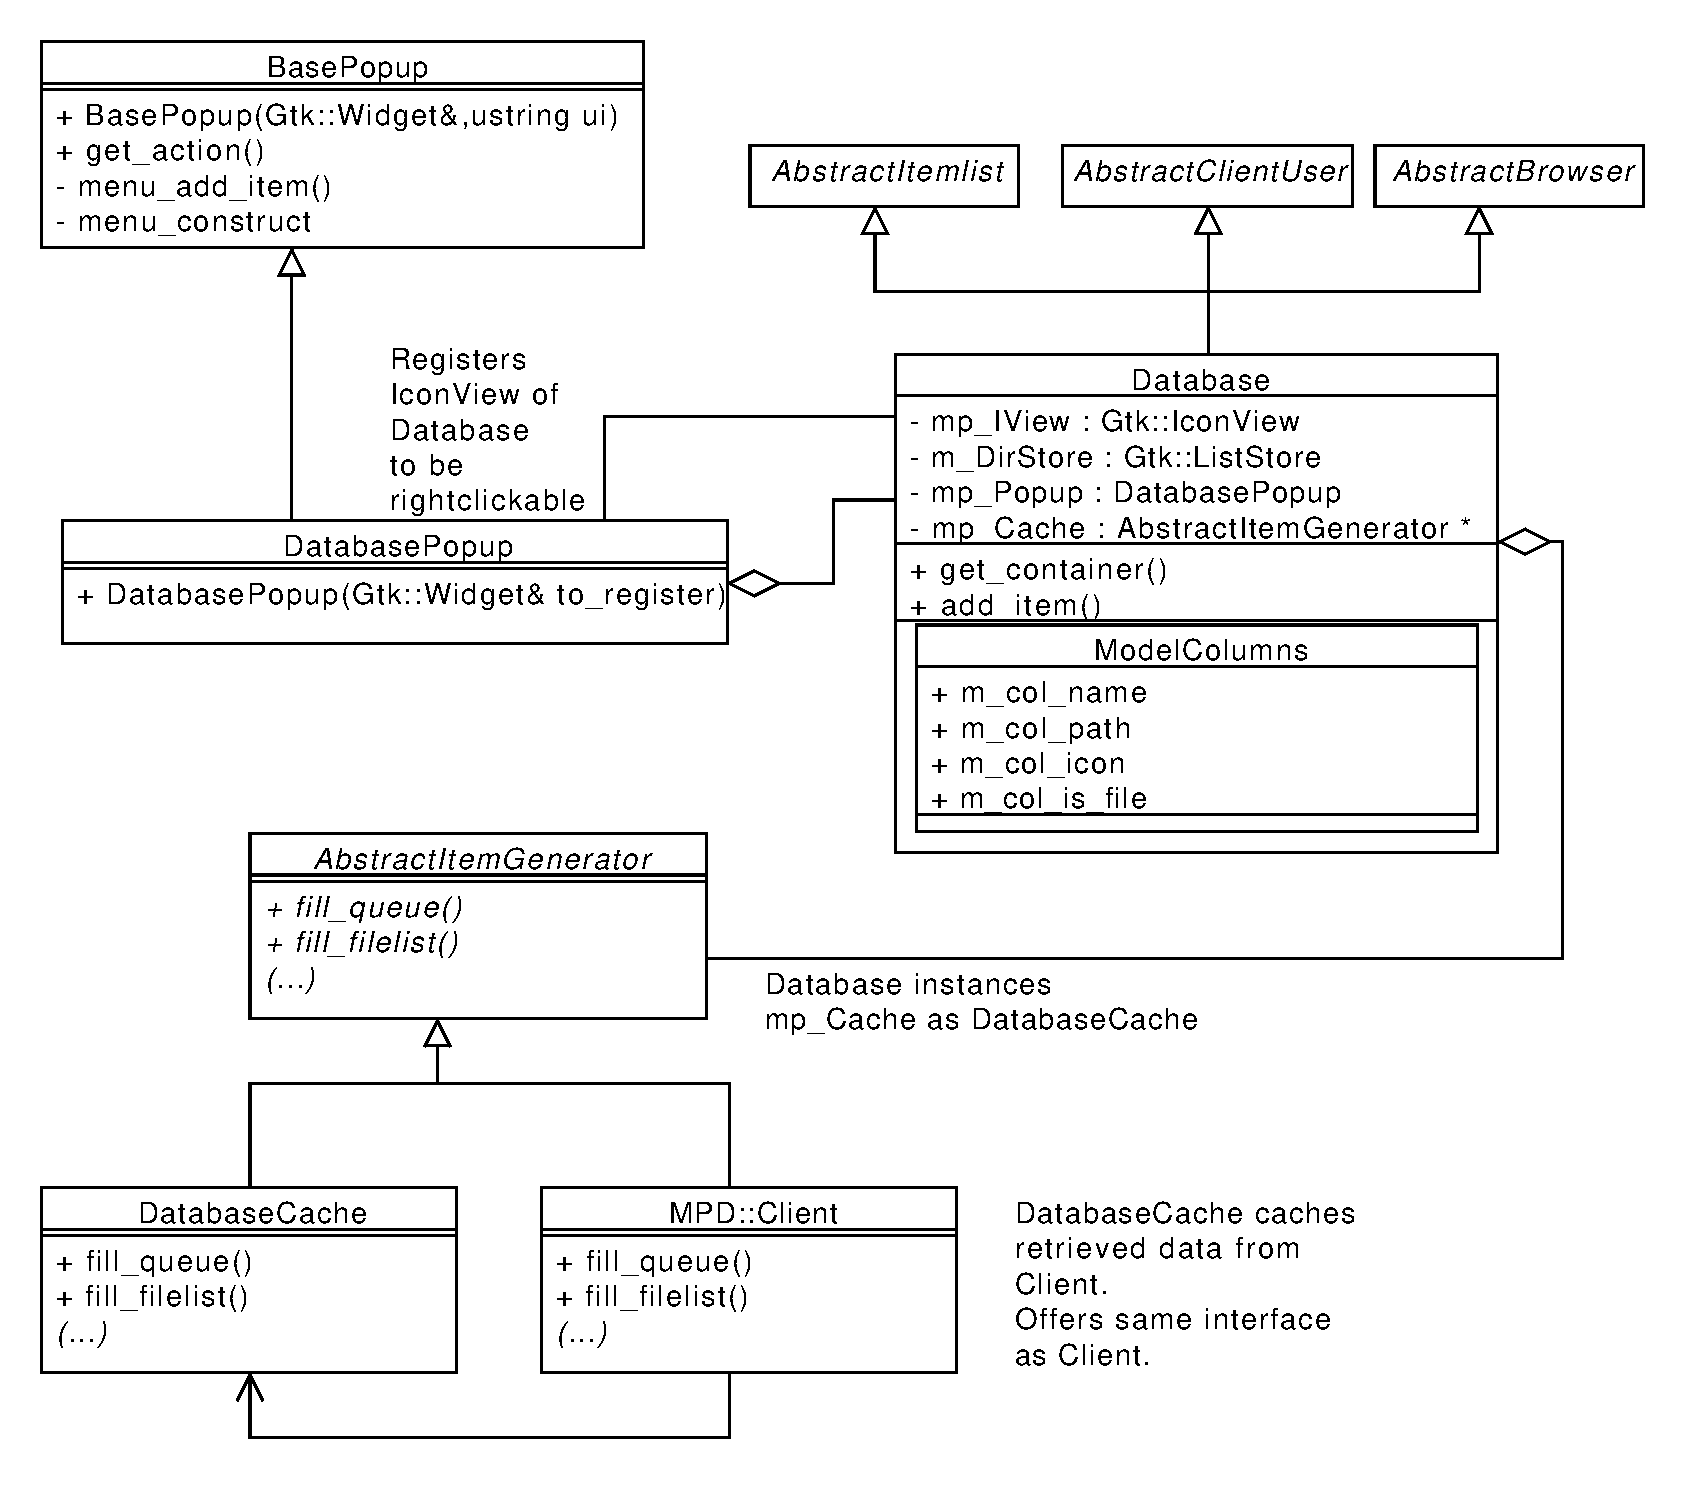
\includegraphics[width=\textwidth]{DatabaseClass.pdf}
	\caption{Klassenübersicht zum Database Browser}
	\label{st_database}
\end{figure}
\paragraph{Database}
Diese Klasse kontrolliert die Anzeige des Datenbankbrowsers. Sie leitet sich daher von \emph{AbstractBrowser} ab um sich bei der Browserliste registrieren zu können.
Um die Methoden des \emph{AbstractItemGenerator} Interface zu benutzen leitet es zudem von \emph{AbstractItemlist} ab und implementiert daher eine add\_item() Methode. 
Diese fügt letzlich die gewonnenen Items seinem Model (einem Gtk::ListStore) hinzu.
Siehe auch \ref{st_database}.
\newpage

\paragraph{DatabasePopup}
Eine Klasse die von BasePopup ableitet und das Popup definiert, das auftaucht wenn man im Databasebrowser ,,rechtsklickt''.
Sie bietet die folgenden Aktionen an, die man über die Methode get\_action() abgefragt werden kann.
Dadurch kann auf folgende Aktionen reagieren kann:
\begin{itemize}
\item ,,db\_add'' (Fügt Auswahl zum Ende der Queue hinzu)
\item ,,db\_add\_all'' (Fügt alles zum Ende der Queue hinzu)
\item ,,db\_replace'' (Dasselbe wie db\_add, leert aber Queue vorher)
\item ,,db\_update'' (Sendet Server einen Updatehinweis)
\item ,,db\_rescan'' (Sendet Server einen Rescanhinweis)
\end{itemize}

\paragraph{DatabaseCache}
Ein Zwischenspeicher für die im Databasebrowser angezeigten Ordner und Dateien. 
Sie setzt das Proxy-Pattern für MPD::Client um und erbt daher von der \emph{AbstractItemGenerator} um sich als Client ausgeben zu können.
Sie implementiert daher die fill\_filelist() Methode vor, lässt aber die anderen Methoden ohne Implementierung.
Da sie auch selbst Daten dem Cache hinzufügen muss leitet sich auch von \emph{AbstractItemlist} ab und implementiert daher auch eine add\_item() Methode. 
\\
Das zugrunde liegende Model ist dabei eine std::map (also eine Art Hashmap) die als Key den Pfad der zu ladenden Seite benutzt
und als Wert ein Vektor von \emph{AbstractComposites} speichert. Wird eine Seite vom ,,Cache'' über die fill\_filelist() Methode verlangt,
so wird nachgeschaut ob im angegeben Pfad bereits eine Seite gespeichert ist, falls nicht wird sie vom Server geholt und gespeichert. 
Anschließend wird über die Elemente iteriert welche durch die add\_item() Methode des Aufrufers weitergegeben werden. 
Sollte sich der Server wechseln bzw. sich die Datenbank aktualisieren, so wird der Cache geleert damit die Anzeige stets aktuell ist. Das MPD Protokoll bietet hier leider keine Möglichkeit rauszufinden was genau sich geändert hat.
\\
\textbf{Anmerkung:} Alle anderen Funktionen von AbstractItemGenerator werden nicht ausimplementiert.

\subsubsection{PlaylistManager}
\paragraph{PlaylistManager}
Diese Klasse kontrolliert die Anzeige des ,,Playlists'' Browsers. Er verwaltet eine Liste der auf dem Server gespeicherten Playlisten. Es soll dabei eine Spalte mit dem Namen und eine Spalte mit dem letzten Änderungsdatum angezeigt werden.
Die Namensspalte soll editierbar sein und nicht prüfen ob der neue Name bereits vorhanden ist. In diesem Falle soll der Editiervorgang nochmal gestartet werden.
Zudem werden die Aktionen des Popupmenüs implementiert.

\paragraph{PlaylistManagerPopup}
Eine Klasse die von BasePopup ableitet und das Popup definiert das auftaucht wenn man im PlaylistManager ,,rechtsklickt''.
Sie bietet die folgenden Aktionen an, die man über die Methode get\_action() abfragen kann und dadurch auf diese Aktionen reagieren kann:
\begin{itemize}
\item pl\_append (Fügt Inhalt der ausgewählten Playlists zum Ende der Queue hinzu)
\item pl\_replace (Dasselbe wie pl\_append, aber leert vorher Queue)
\item pl\_delete (Löscht Playliste aus der Liste und vom Server)
\end{itemize}

\subsubsection{Queue}
\begin{figure}[htb!]
	\centering
        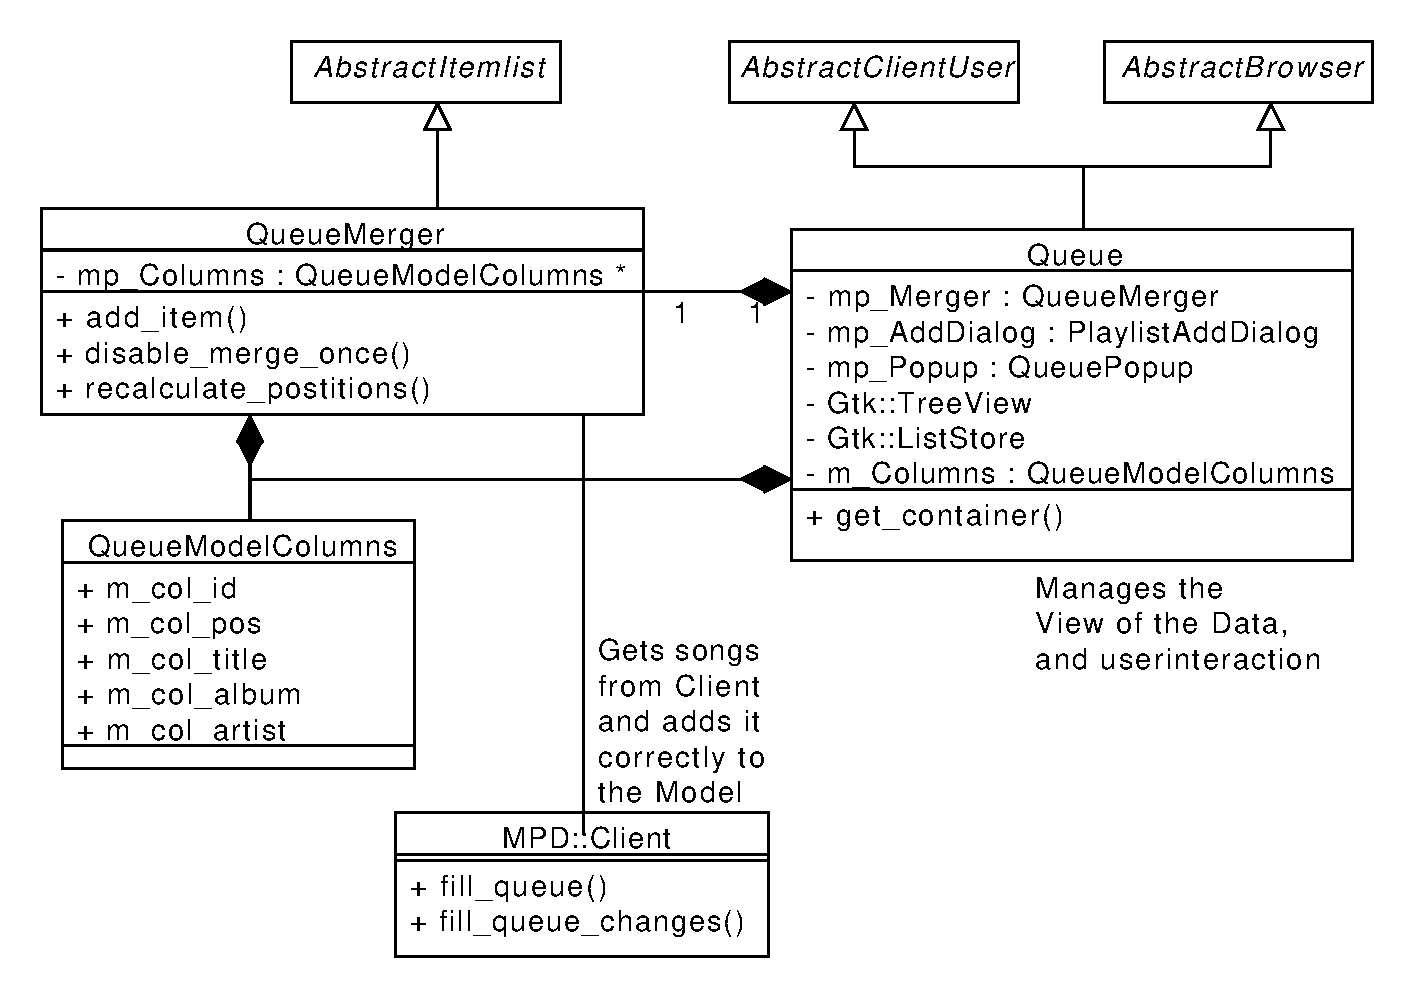
\includegraphics[width=\textwidth]{QueueClass.pdf}
	\caption{Klassenübersicht zur Queue}
	\label{st_queue}
\end{figure}
\newpage
\paragraph{Queue}
Diese Klasse kontrolliert die Anzeige der Queue (der aktuellen Playlist) und auch die Verwaltung des darunter liegenden Suchfelds.
(Siehe auch \ref{st_queue})
\\
\\
\textbf{Suchfunktion:} Beim Tippen soll zum Künstler in der Liste gesprungen werden der mit den getippten Buchstaben beginnt.
,,Kno'' sollte also zu ,,Knorkator'' springen. Bei Aktivierung des Suchfelds muss die Auswahl entsprechend einer Volltextsuche gefiltert werden. Durch Aktivieren der Tastenkombination \textit{Ctrl-F} soll zudem der Fokus auf das Suchfeld gelegt werden.
Zudem werden folgende Aktionen des Popupmenüs implementiert:
\begin{itemize}
\item Remove - Entfernt ausgewählte Elemente aus der Queue und benachrichtigt Server.
\item Clear - Leert alle Daten aus dem Model und benachrichtigt den Server entsprechend
\item Save as Playlist - Speichert aktuellen Inhalt als Playliste; Namensabfrage durch PlaylistAddDialog
\end{itemize}

Das zugrundeliegende Model ist ein Gtk::ListStore dessen Spaltenlayout durch QueueModelColumns festgelegt wird.
Als View wird ein Gtk::TreeView verwendet.

\paragraph{QueueModelColumns}
Definiert die Spalten für die Queue, und erbt daher von Gtk::TreeModel::ColumnRecord, sodass ein Gtk::ListStore etwas damit anfangen kann.
Die Definition ist nicht wie bei anderen Klassen als ,,Nested Class'' realisiert, da sowohl Queue als auch QueueMerger darauf zugreifen müssen. 
Sie definiert die folgenden Spalten:
\begin{itemize}
\item m\_col\_id: Speichert die Songid eines Songs (nicht sichtbar)
\item m\_col\_pos: Speichert die Position eines Songs (beginnend bei 0) (nicht sichtbar)
\item m\_col\_title: Der Songtitel
\item m\_col\_album: Der Albumtitel
\item m\_col\_artist: Der Artisttitel
\end{itemize}

\paragraph{QueueMerger}
Diese Klasse verwaltet die eigentlichen Daten die die Queue anzeigt.
Sie soll ihre Daten vom Client beziehen und erbt daher von \emph{AbstractItemlist} wodurch 
eine add\_item() Methode implementiert werden muss. Da sie die Änderungen auch in die Queue einpflegen muss, erwartet die ,,Merger'' Klasse eine Referenz auf das der Queue zugrunde liegende Gtk::ListStore Model, sowie deren Spaltendefinition die als drittes Argument übergeben werden muss:
\begin{verbatim}         
      QueueMerger(MPD::Client& client,
                  Glib::RefPtr<Gtk::ListStore>& queue_model,
                  QueueModelColumns& queue_columns);
\end{verbatim}

QueueMerger soll die folgenden \textit{public} Funktionen bieten:
\\
disable\_merge\_once() lässt das ,,Zusammenführen'' einmal ausfallen. Dies ist nützlich bei der Implementierung der ,,Remove'' Funktionalität,
da man weiß wo ein Element gelöscht wurde, und es so aus Performancegründen explizit aus View und Model entfernen kann.
\begin{verbatim}  
    void disable_merge_once(void);
\end{verbatim}
recalulate\_positions() kann nützlich im Zusammenhang mit disable\_merge\_once() sein. Löscht man etwas explizit, so ist die Spalte mit den Positionsangaben korrumpiert. Diese Funktion berechnet die Positionen angefangen bei ,,pos'' neu.
\begin{verbatim}        
    void recalculate_positions(unsigned pos = 0);
\end{verbatim}    

Bei einem Clientupdate sollen Änderungen über die Clientmethode fill\_queue\_changes() vom Server geholt und in die Queue eingepflegt werden. 

%<Zustandsdiagramm mit weiterer Auarbeitung hier>

\paragraph{QueuePopup}
Eine Klasse die von BasePopup ableitet und das Popup definiert das auftaucht wenn man in der Queue ,,rechtsklickt''.
Sie bietet die folgenden Aktionen an die man über die Methode get\_action() abfragen kann und dadurch auf diese Aktionen reagieren kann:
\begin{itemize}
\item q\_remove (Entfernt ausgewählte Elemente aus der Queue)
\item q\_clear (Leert Queue völlig)
\item q\_add\_as\_pl (Zeigt den PlaylistAddDialog)
\end{itemize}

\paragraph{PlaylistAddDialog}
Zeigt einem Dialog zum Speichern der aktuellen Queue als Playlist mit einem bestimmten Namen. Der Name wird durch den Dialog abgefragt.
Es wird keine Validierung durchgeführt, außer dass der Name länger als ein 0 Zeichen sein muss. Der eingegebene Name soll an den Aufrufer zurückgegeben werden.

\newpage
\subsubsection{Settings}
\paragraph{AbstractSettings}
\begin{figure}[htb!]
	\centering
        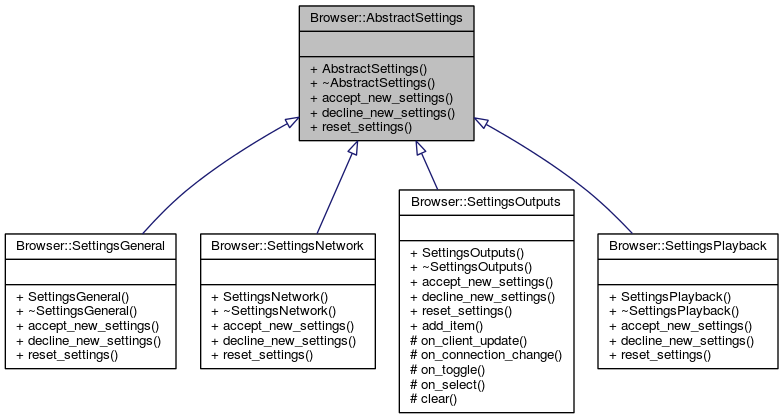
\includegraphics[scale=0.5]{AbstractSettings.png}
	\caption{Nutzer von AbstractSettings}
	\label{class_abstract_browser}
\end{figure}
Eine abstrakte Klasse die einen Reiter im Settingsbrowser repräsentiert. 
Sie soll die folgenden ,,pure virtual'' Methoden definieren:

\begin{verbatim}
    virtual void accept_new_settings(void)
\end{verbatim}
Weist Reiter an, alle Werte in die Config zu speichern     
\begin{verbatim}
    virtual void decline_new_settings(void)
\end{verbatim}     
Weist Reiter an, die letzten validen Werte aus der Config zu laden

\begin{verbatim}
    virtual void reset_settings(void)
\end{verbatim}
Weist Reiter an, die Defaultwerte aus der einkompilierten Config zu laden.

\newpage

\paragraph{Settings}
\begin{figure}[htb!]
	\centering
        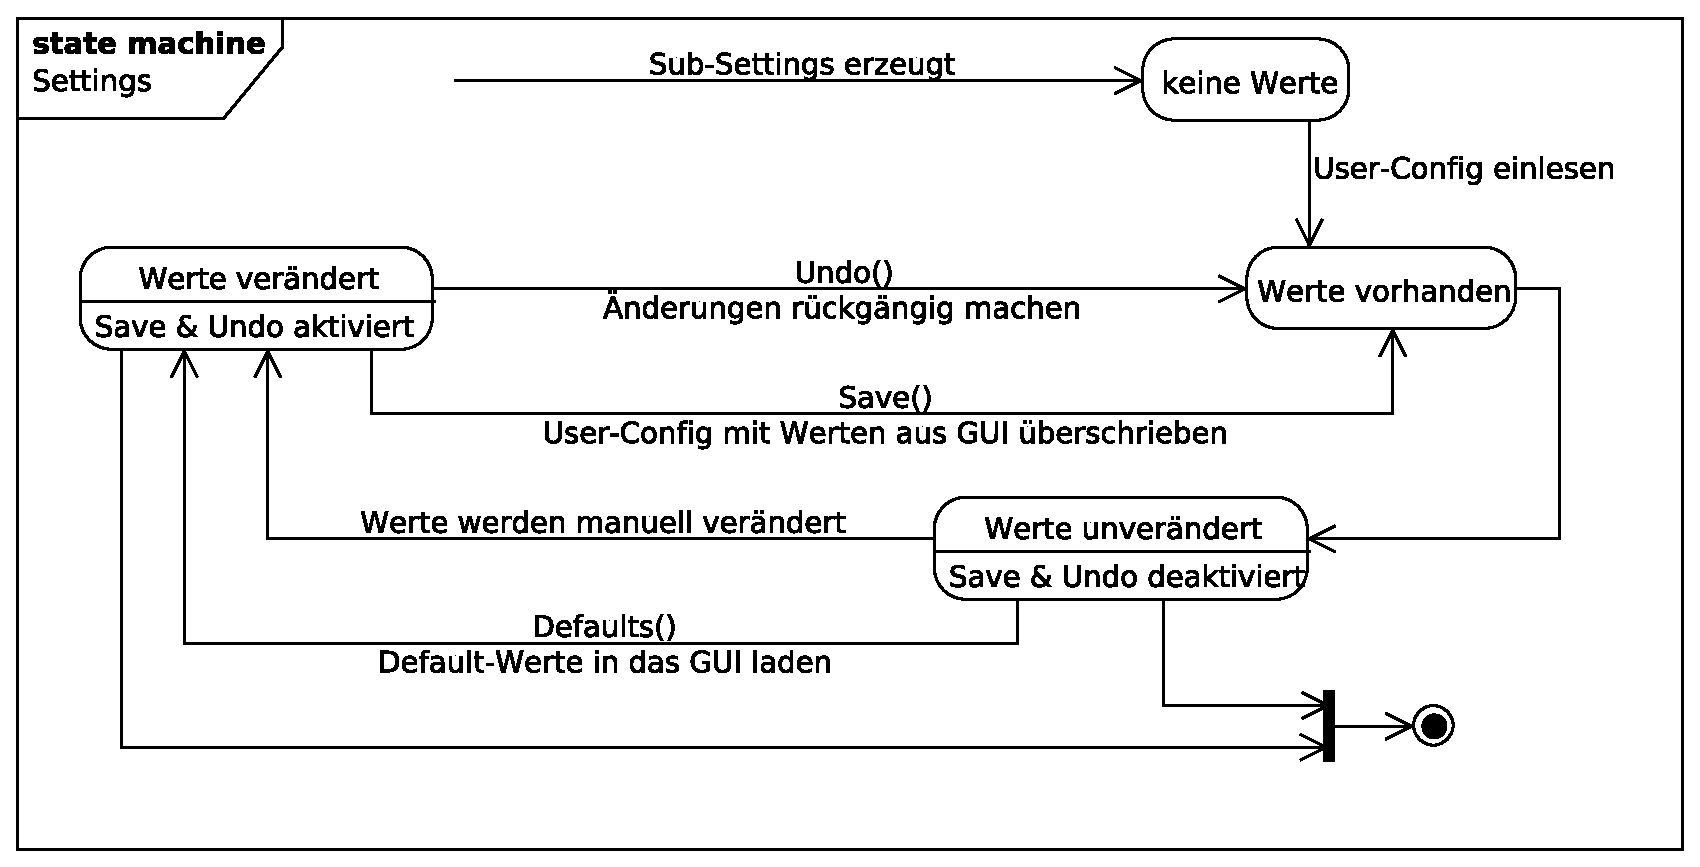
\includegraphics[width=\textwidth]{st_Settings.eps}
	\caption{Zustandsdiagramm Settings}
	\label{st_settings}
\end{figure}
Die Settings Klasse repräsentiert den Settingsbrowser. Wie jeder andere Browser implementiert diese Klasse \emph{AbstractBrowser} und eine get\_container() Methode.
Sobald etwas in der Präsentation geändert wird, soll es nicht gleich in die Config übernommen werden.
Dies soll erst durch den Speicherbutton geschehen (siehe \ref{st_settings}).
\begin{itemize}
\item Zurücksetzen - Setzt alle Einstellungen auf Fabrikstandards zurück
\item Rückgängig - Setzt Änderungen auf letzten Stand zurück
\item Speichern - Speichert aktuelle Änderungen
\end{itemize}

Die Klasse soll zudem eine Methode bieten um anzuzeigen, dass die ,,Settings'' geändert wurden z.B. durch Ausgrauen des Speicherbuttons:
\begin{verbatim}
    void settings_changed(void)
\end{verbatim}
Um in jeden Tab die Settings zurückzusetzen (auf letzten validen Wert oder Standardwert) speichert die Settingsklasse für jeden Reiter eine AbstractSettings Instanz in eine Liste. Sie kann so später darüber iterieren um die werte zu speichern, rückgängig zu machen oder zurück zu setzen. 

%<Zustandsdiagramm zum Settings akzeptieren, sprich buttons in/sens machen>

\paragraph{Settings}
\begin{figure}[htb!]
	\centering
        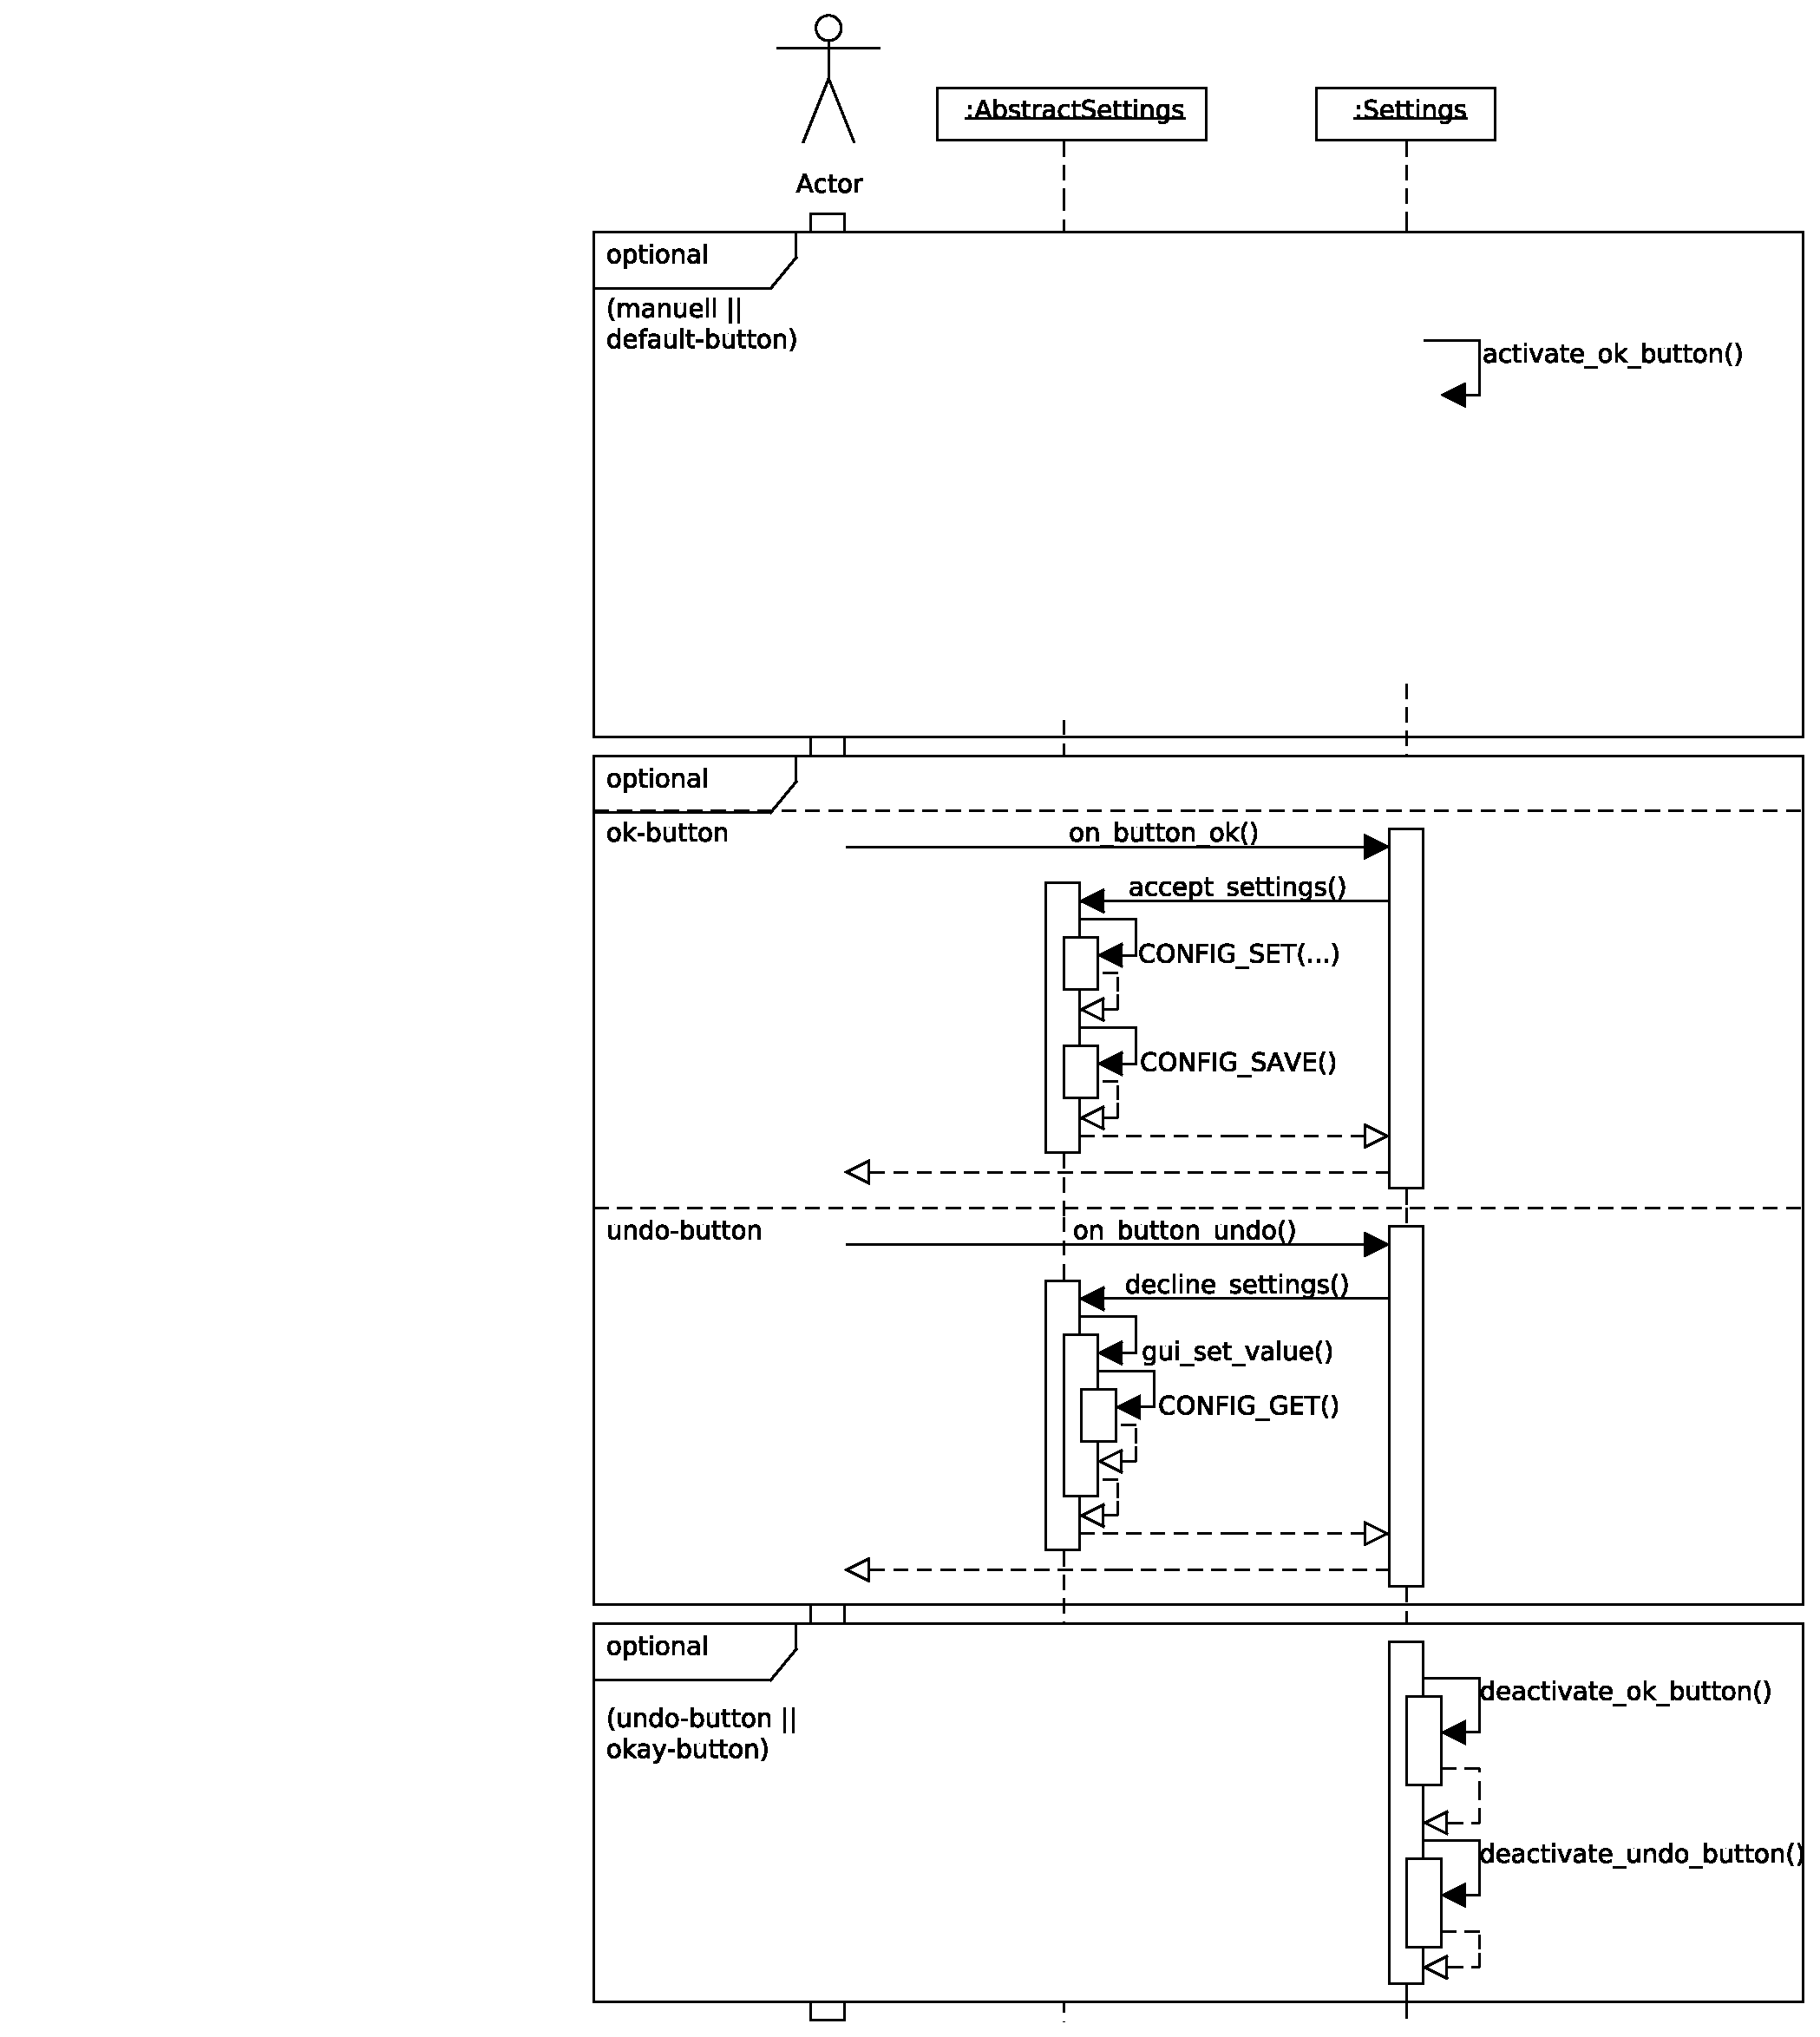
\includegraphics[scale=0.52]{st_settings2.eps}
	\caption{Settings Sequenzdiagramm}
	\label{st_seq_settings}
\end{figure}


\paragraph{SettingsGeneral}
Die konkrete Klasse die den ,,General'' Tab implementiert.
Folgende Einstellungen sollen geändert werden können:
\begin{itemize}
\item ,,settings.libnotify.signal'' (checkbox)
\item ,,settings.libnotify.timeout'' (numberslider) (ausgegraut wenn 'signal' nicht aktiviert)
\item ,,settings.trayicon.tray'' (checkbox)
\item ,,settings.trayicon.totrayonclose'' (checkbox) (ausgegraut wenn 'tray' nicht aktiviert)
\end{itemize}

\paragraph{SettingsNetwork}
Die konkrete Klasse die den ,,Network'' Tab implementiert.
Folgende Einstellungen sollen geändert werden können:
\begin{itemize}
\item ,,settings.connection.port'' (numberslider)
\item ,settings.connection.host'' (stringentry)
\item ,,settings.connection.autoconnect'' (checkbox)
\item ,,settings.connection.timeout'' (numberslider)
\item ,,settings.connection.reconnectinterval'' (numberslider)
\end{itemize}
Zusätzlich soll ein Button zum Zeigen der Avahi-Serverliste angezeigt werden.

\paragraph{SettingsPlayback}
Die konkrete Klasse die den ,,Playback'' Tab implementiert.
Folgende Einstellungen sollen geändert werden können:
\begin{itemize}
\item Eine Einstellung zum ,,Crossfade'' (Überblendzeit). Diese wird vom Server gespeichert.
\item ,,settings.playback.stoponexit'' (checkbox)
\end{itemize}

\paragraph{SettingsOutputs}
Zeigt und verwaltet eine Liste von Outputs. Die Klasse benutzt die Funktion \textit{fill\_outputs()} von \emph{AbstractItemGenerator}
und muss daher von AbstractItemlist erben.

Wenn Änderungen übernommen werden, so wird über die Liste iteriert und für jeden Output entsprechend \emph{enable()} oder \emph{disable()} aufgerufen, 
falls der Output vorher aus-, respektive eingeschalten war.

\paragraph{OutputsModelColumns}
Die Spaltendefinition für die Outputliste.
Die Liste besteht aus dem Outputnamen (einem String), einer Anzeige ob der Aktiv ist (boolean),
und einen Pointer auf die AudioOutput Instanz um den entsprechenden Output en/disablen zu können.

\subsubsection{Statistics}
\paragraph{Statistics}
Eine Browserklasse die lediglich eine Reihe von Labels verwaltet und sie bei einem Clientupdate mit den aktuellen Server Statistiken.

Folgende ,,Statistics'' soll die Klasse darstellen:
\begin{itemize}
\item ,,Number of artists'' - Anzahl der Künstler in der Datenbank
\item ,,Number of albums'' - Anzahl der Alben in der Datenbank
\item ,,Number of songs'' - Anzahl der Songs in der Datenbank
\item ,,DB Playtime'' - Gibt die gesamte Spielzeit der Datenbank an
\item ,,Playtime'' - Seit wann abgespielt wird
\item ,,Uptime'' - Gibt an wie lange der Server läuft
\item ,,Most recent db update'' - Aktuellstes Datenbankupdate
\end{itemize}

Diese Informationen werden beim Start des Freya Clients und bei jedem Datenbankupdate abgerufen.

